%% The "\appendix" call has already been made in the declaration
%% of the "appendices" environment (see thesis.tex).
\chapter{Envelope function choices}
\label{sec:app_env}

The invariant mass distributions with the different envelope functions used, after having been fit to the data, for each of the analysis categories in the \MFM analysis.

\begin{figure}
  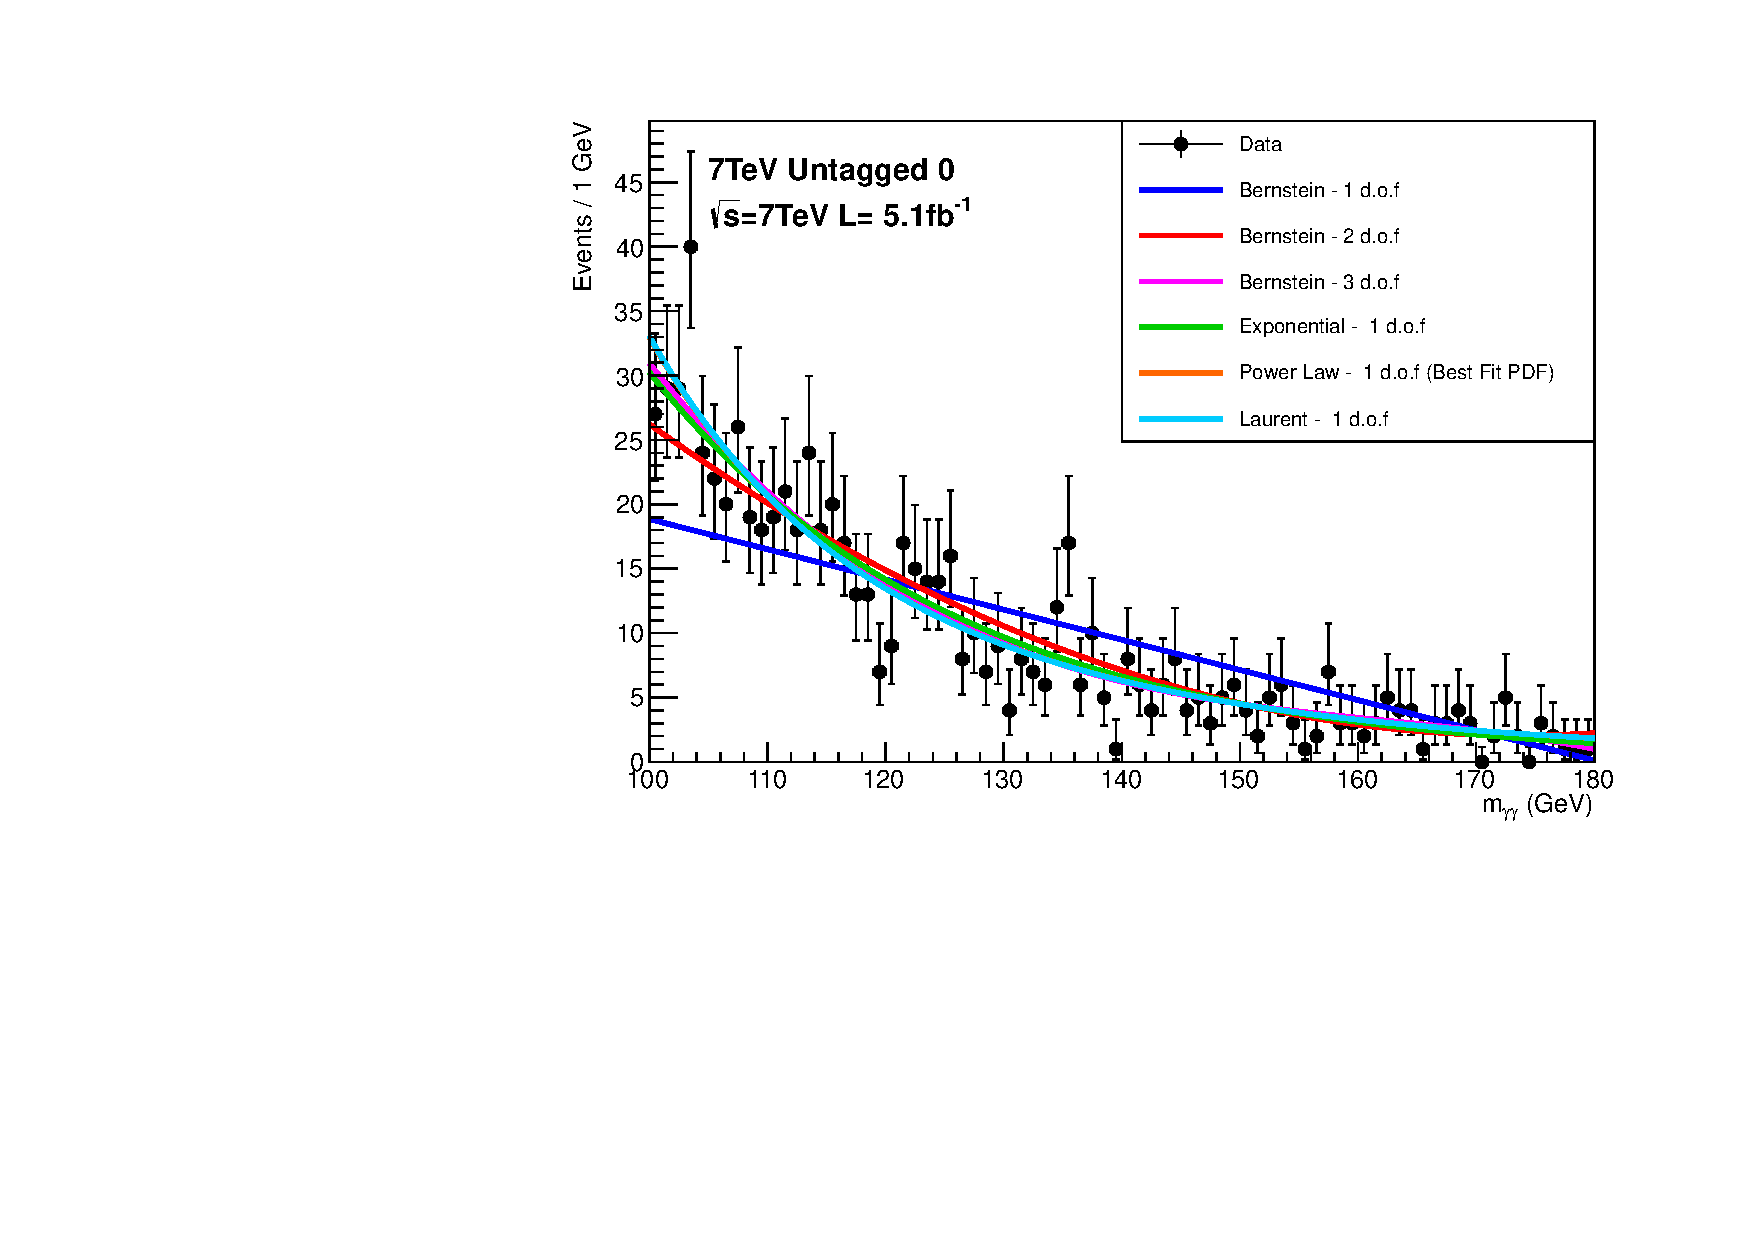
\includegraphics[width=0.49\textwidth]{analysis/plots/multipdf_plots/cat0_7TeV.pdf}
  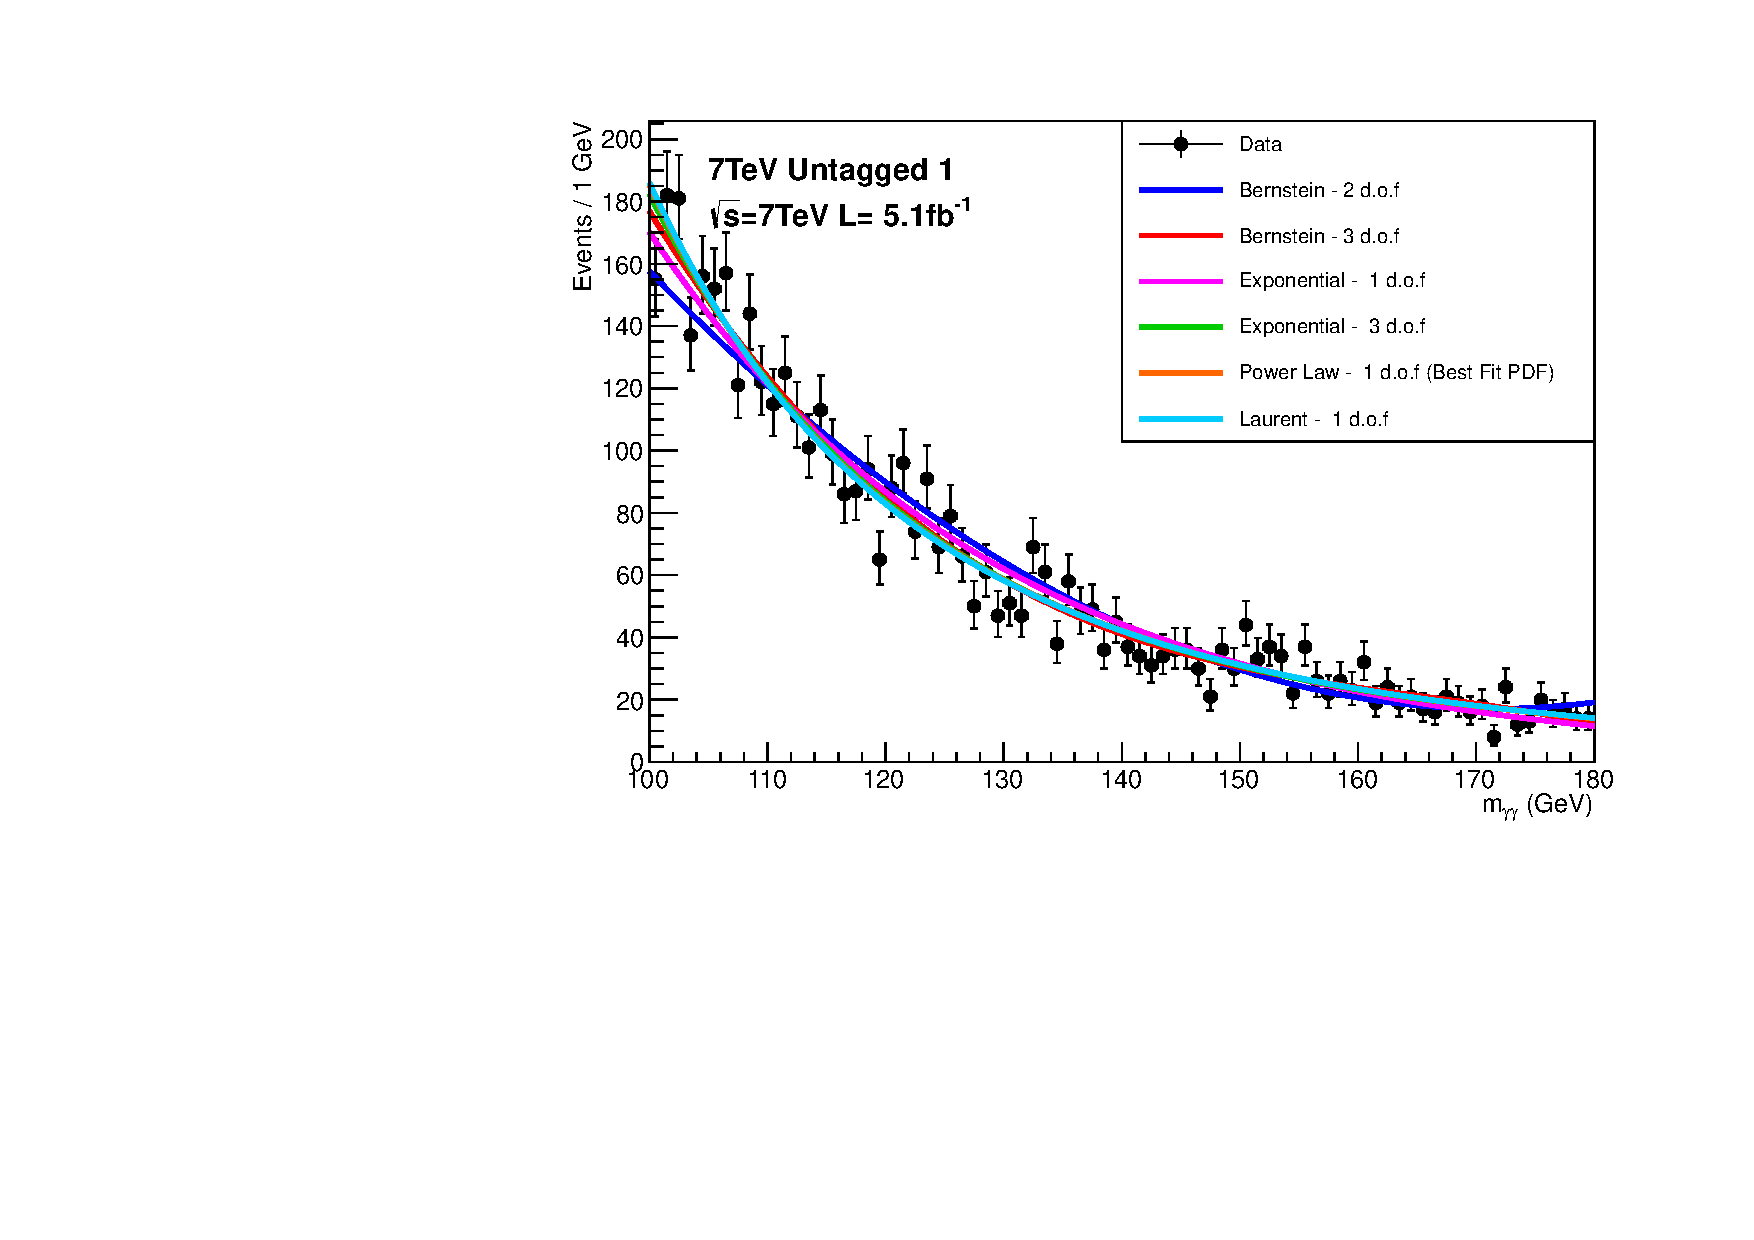
\includegraphics[width=0.49\textwidth]{analysis/plots/multipdf_plots/cat1_7TeV.pdf}\\
  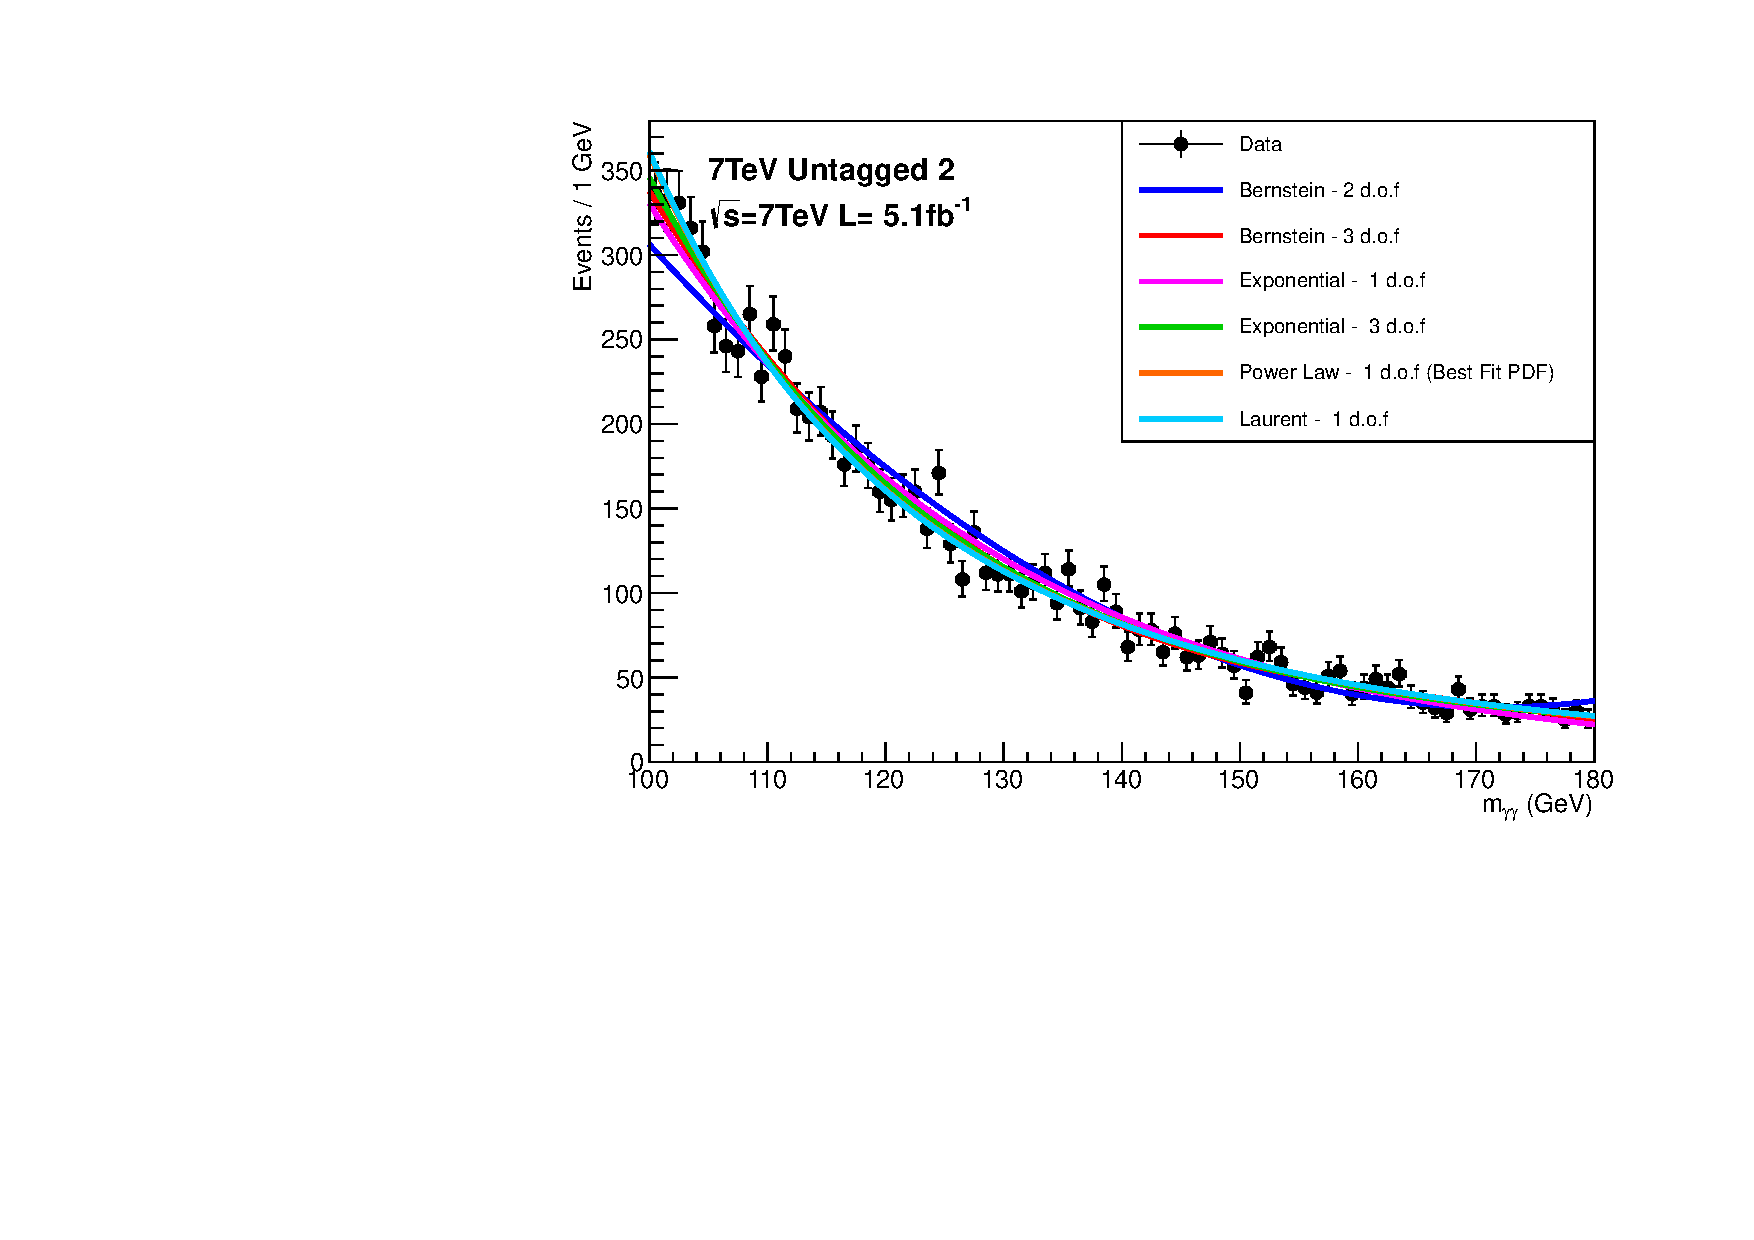
\includegraphics[width=0.49\textwidth]{analysis/plots/multipdf_plots/cat2_7TeV.pdf}
  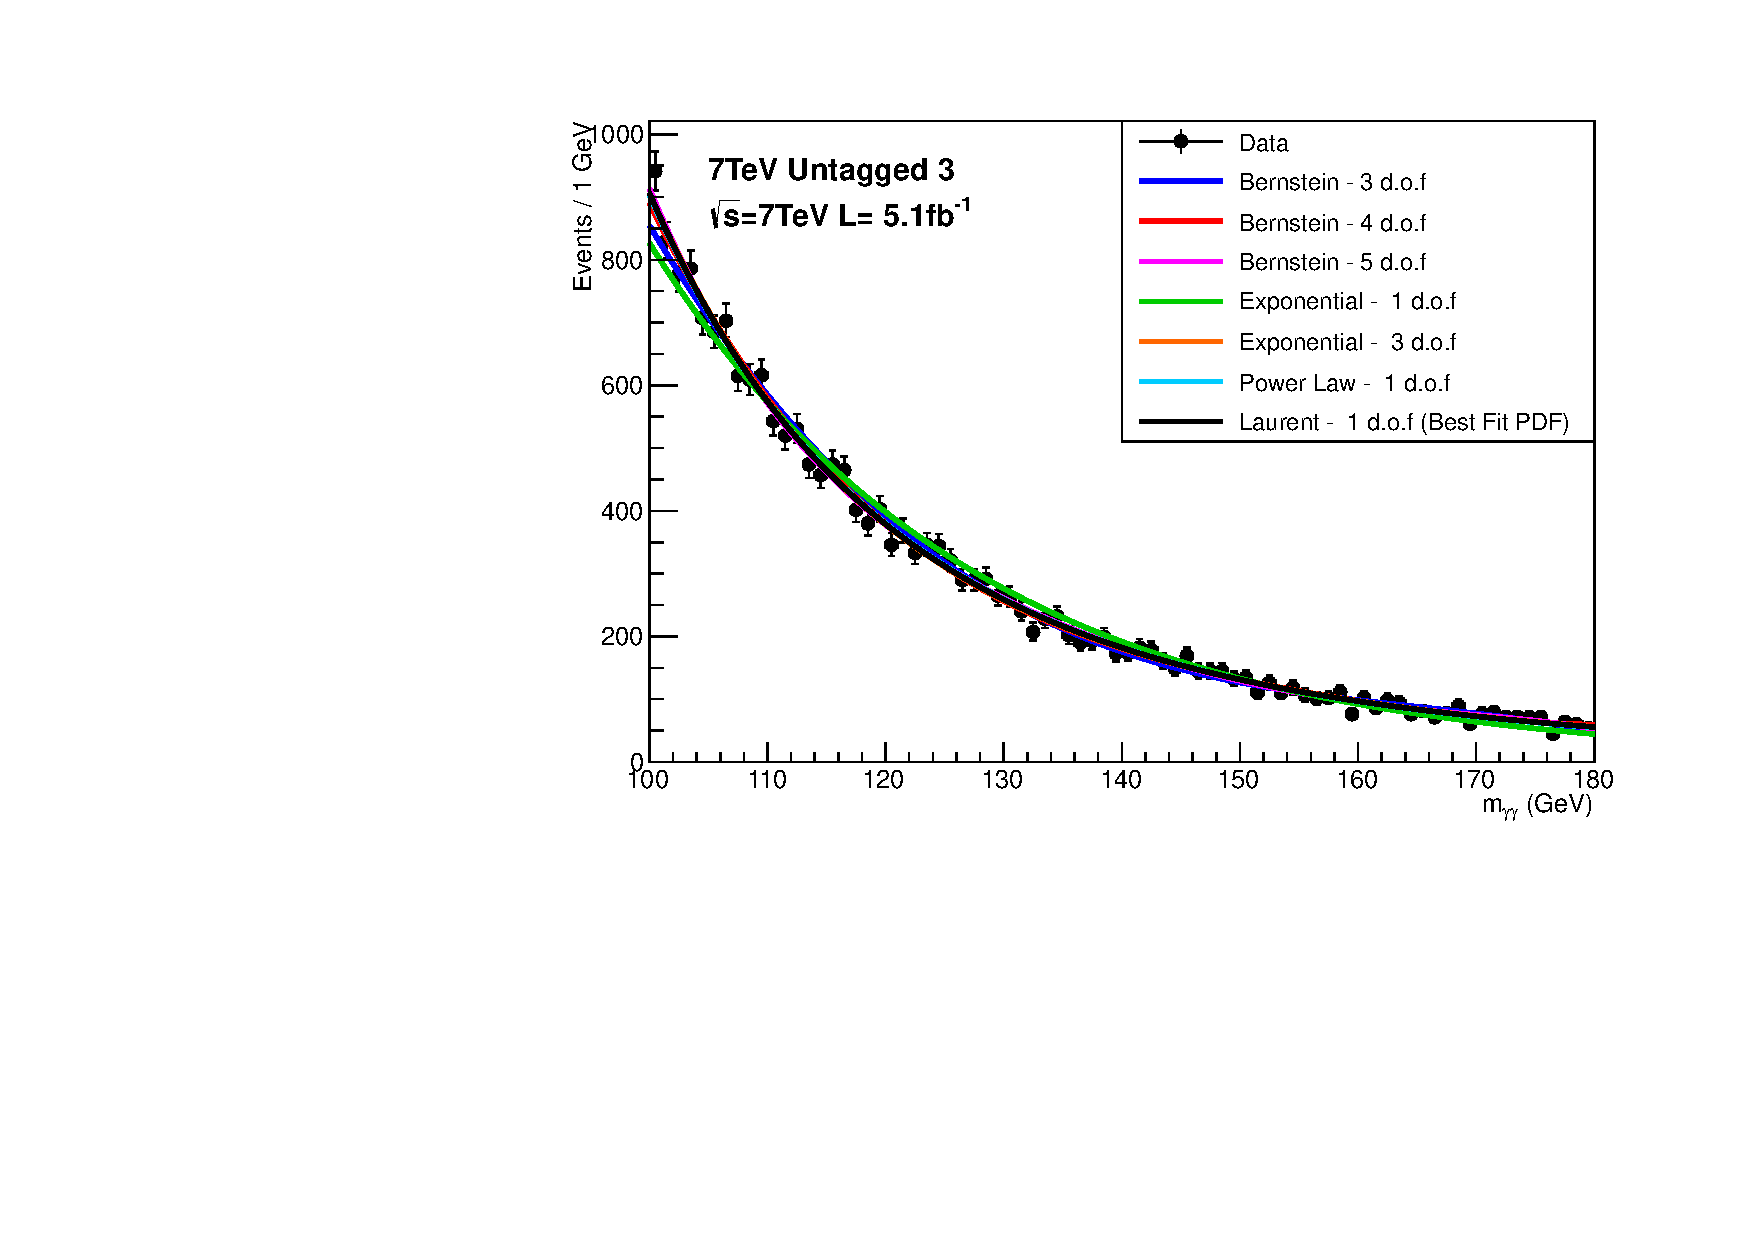
\includegraphics[width=0.49\textwidth]{analysis/plots/multipdf_plots/cat3_7TeV.pdf}\\
  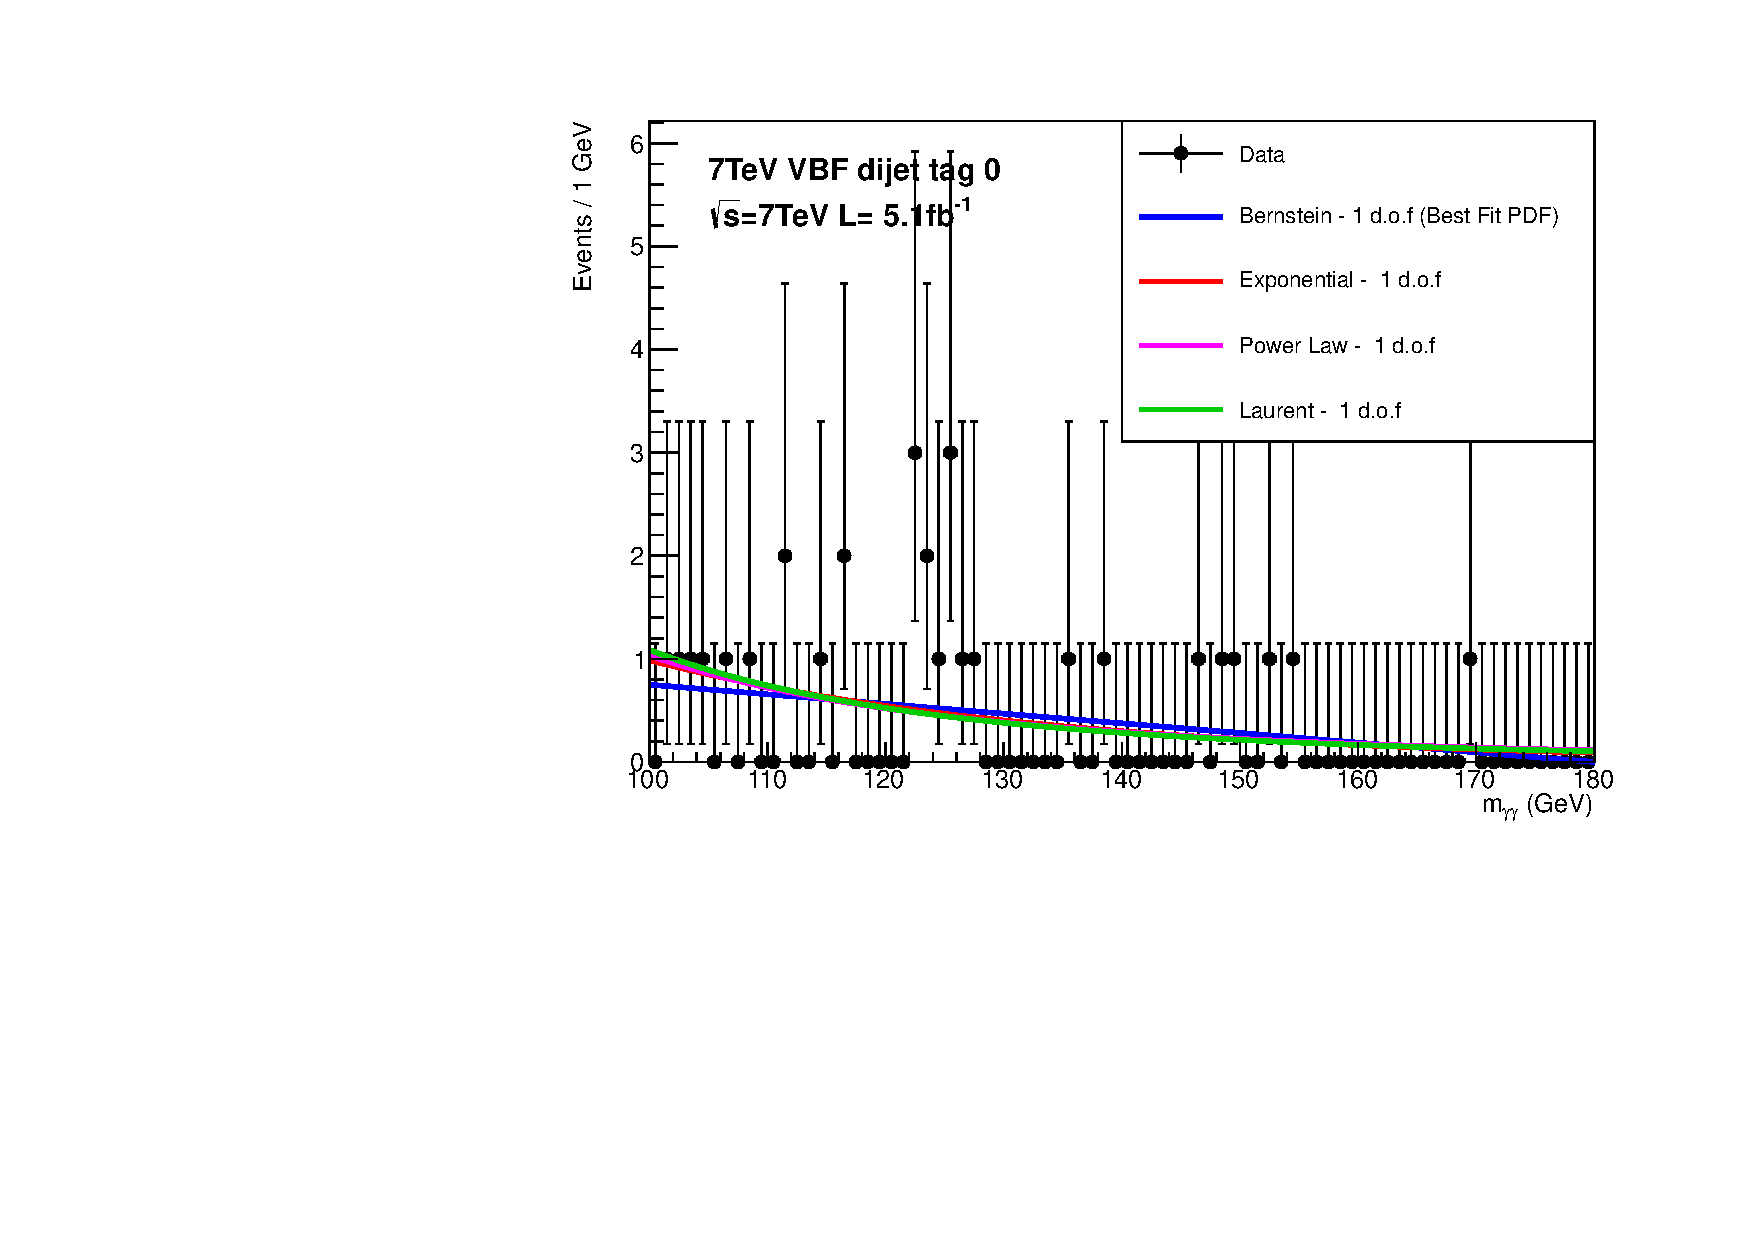
\includegraphics[width=0.49\textwidth]{analysis/plots/multipdf_plots/cat4_7TeV.pdf}
  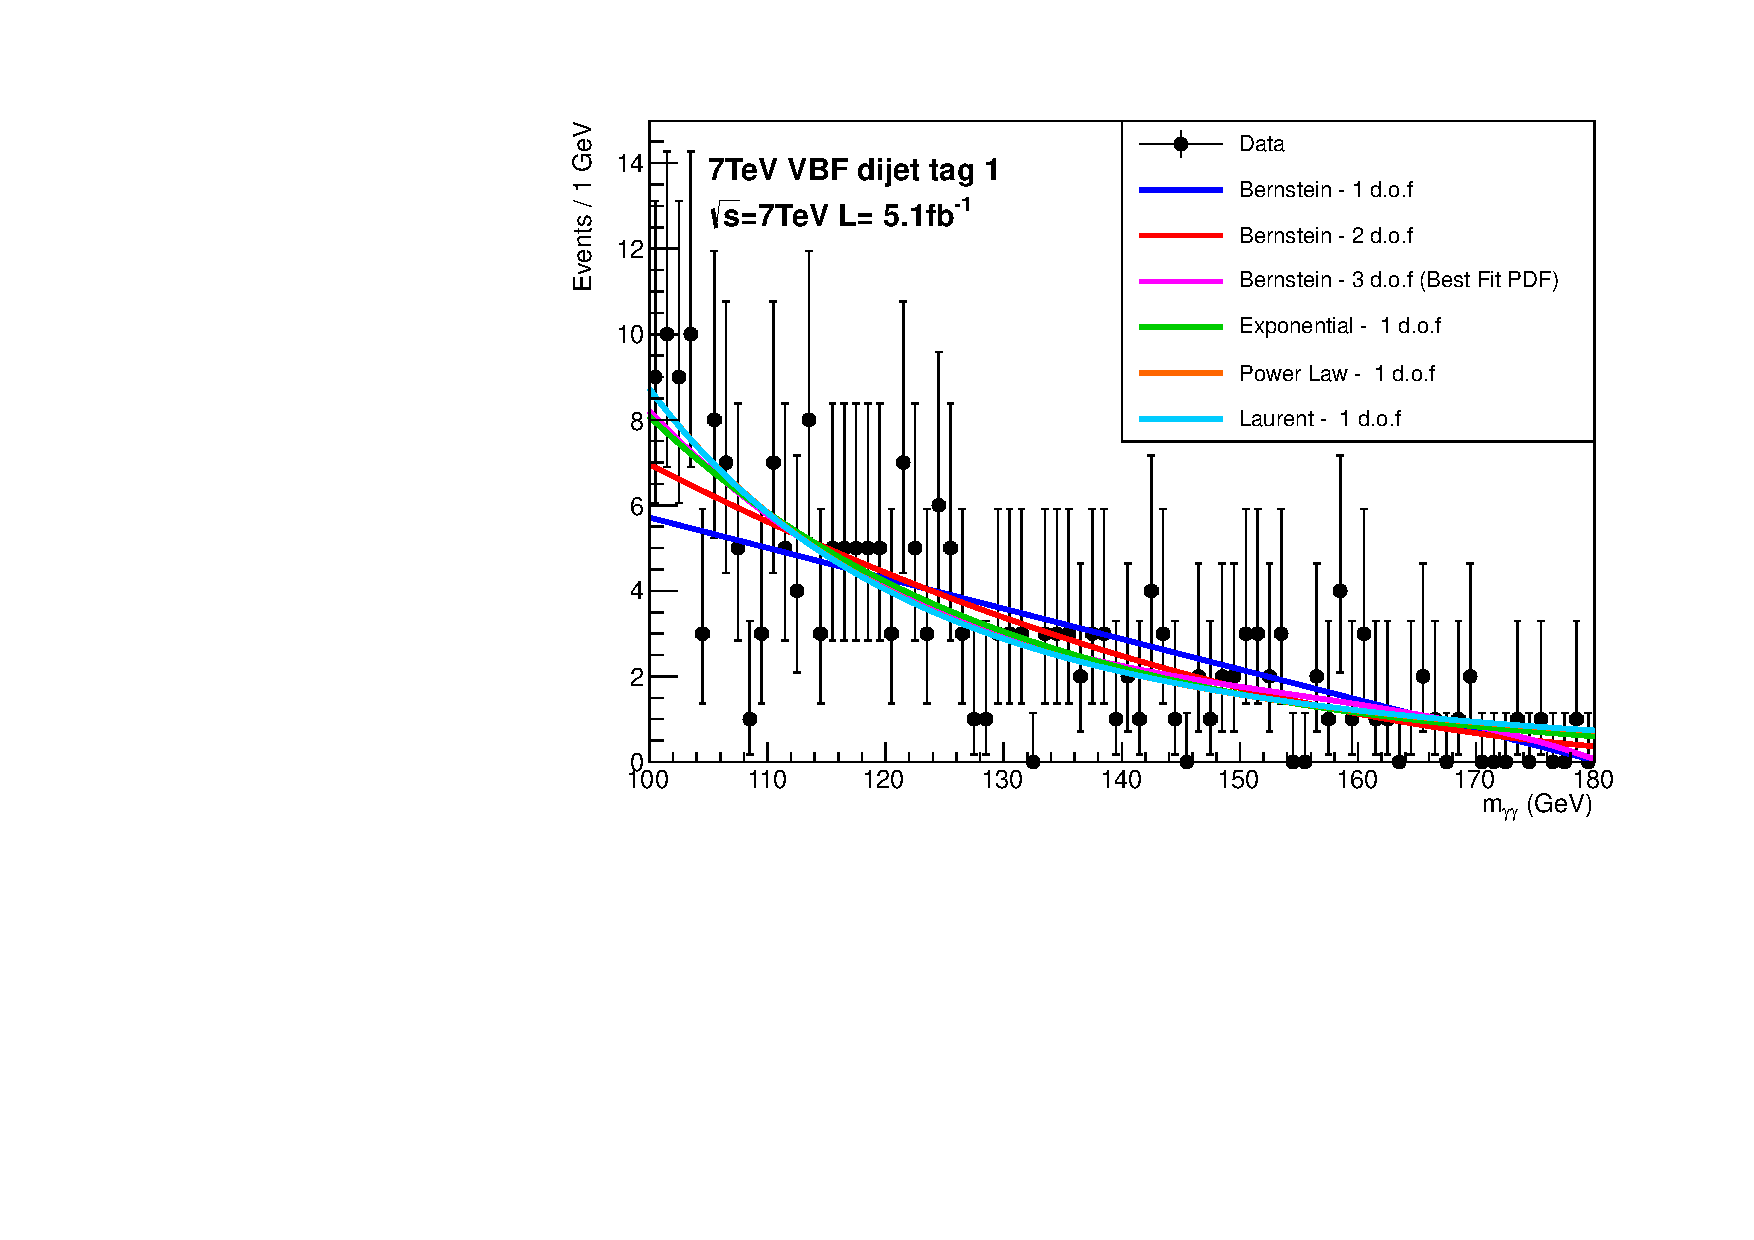
\includegraphics[width=0.49\textwidth]{analysis/plots/multipdf_plots/cat5_7TeV.pdf} \\
  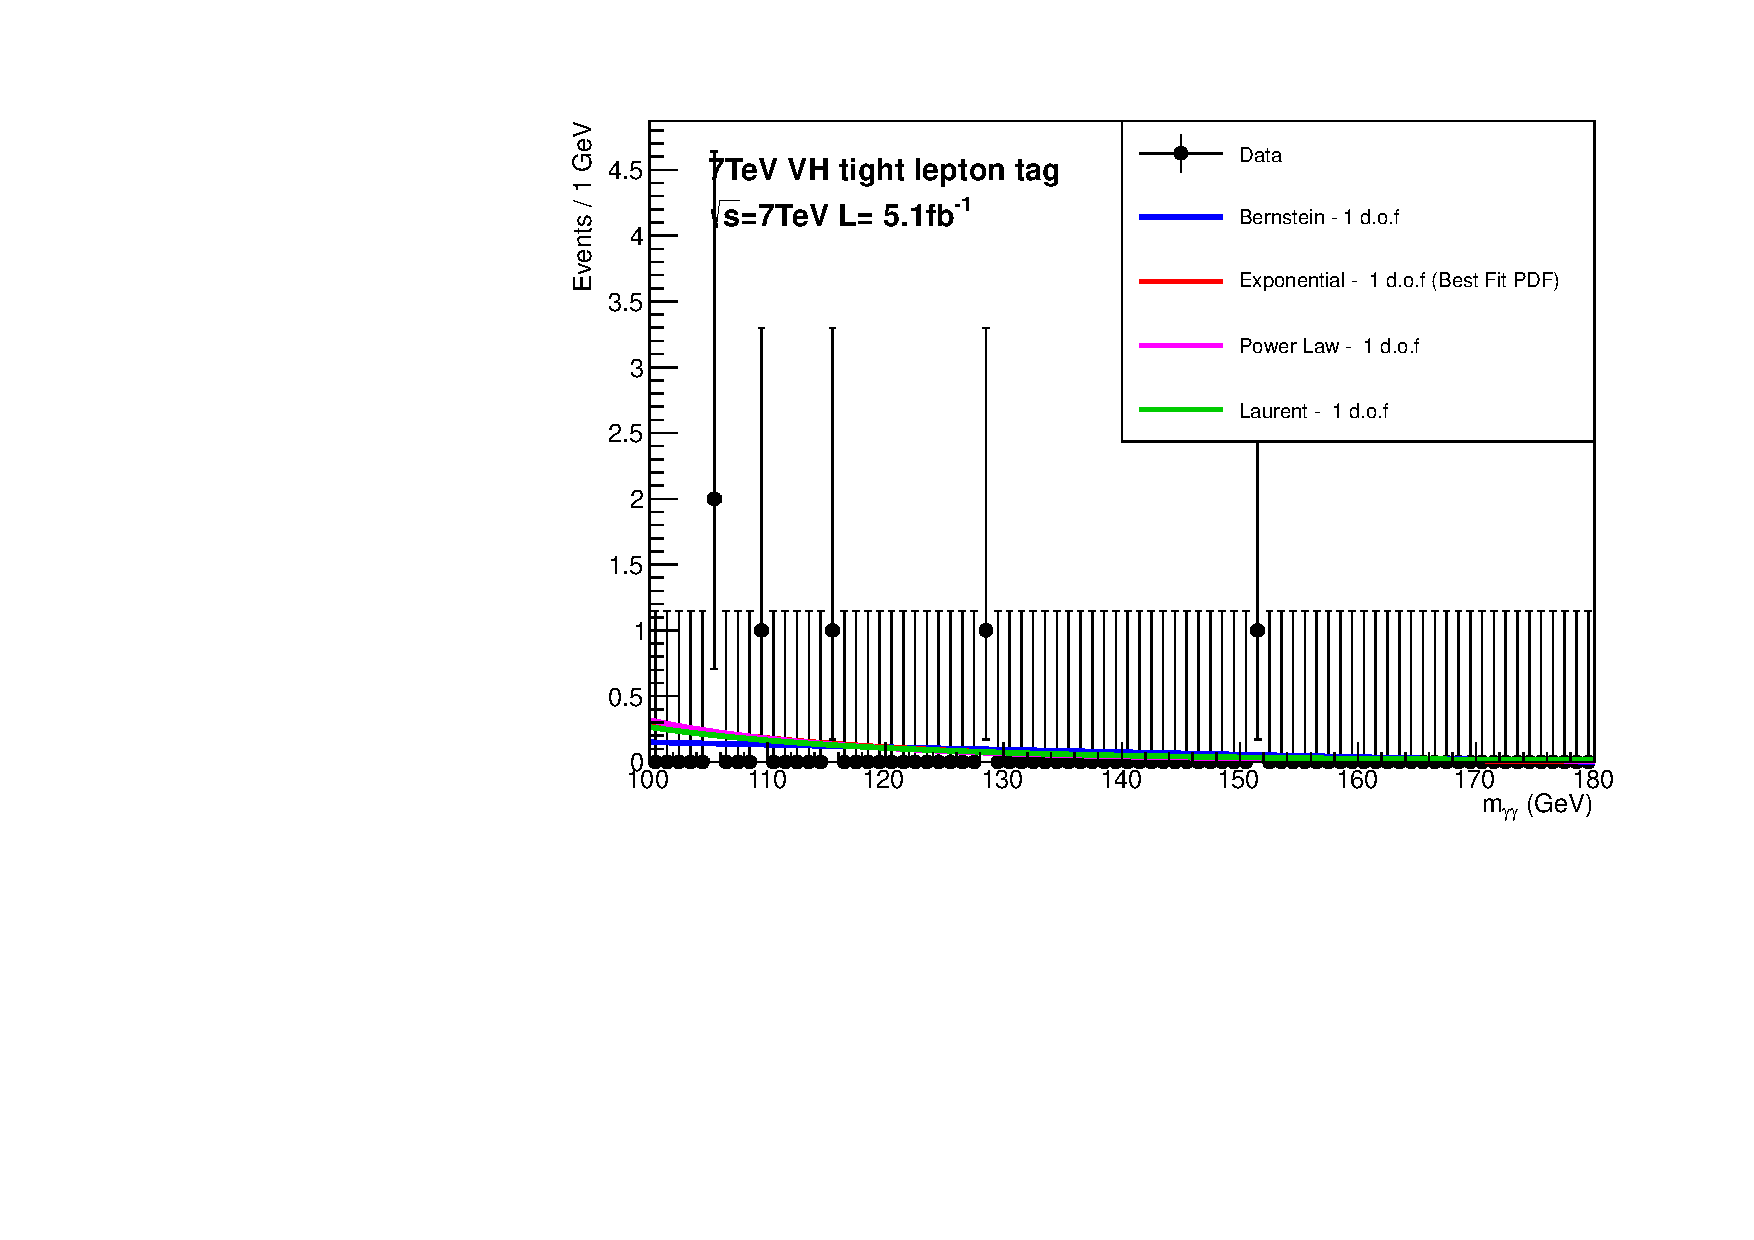
\includegraphics[width=0.49\textwidth]{analysis/plots/multipdf_plots/cat6_7TeV.pdf}
  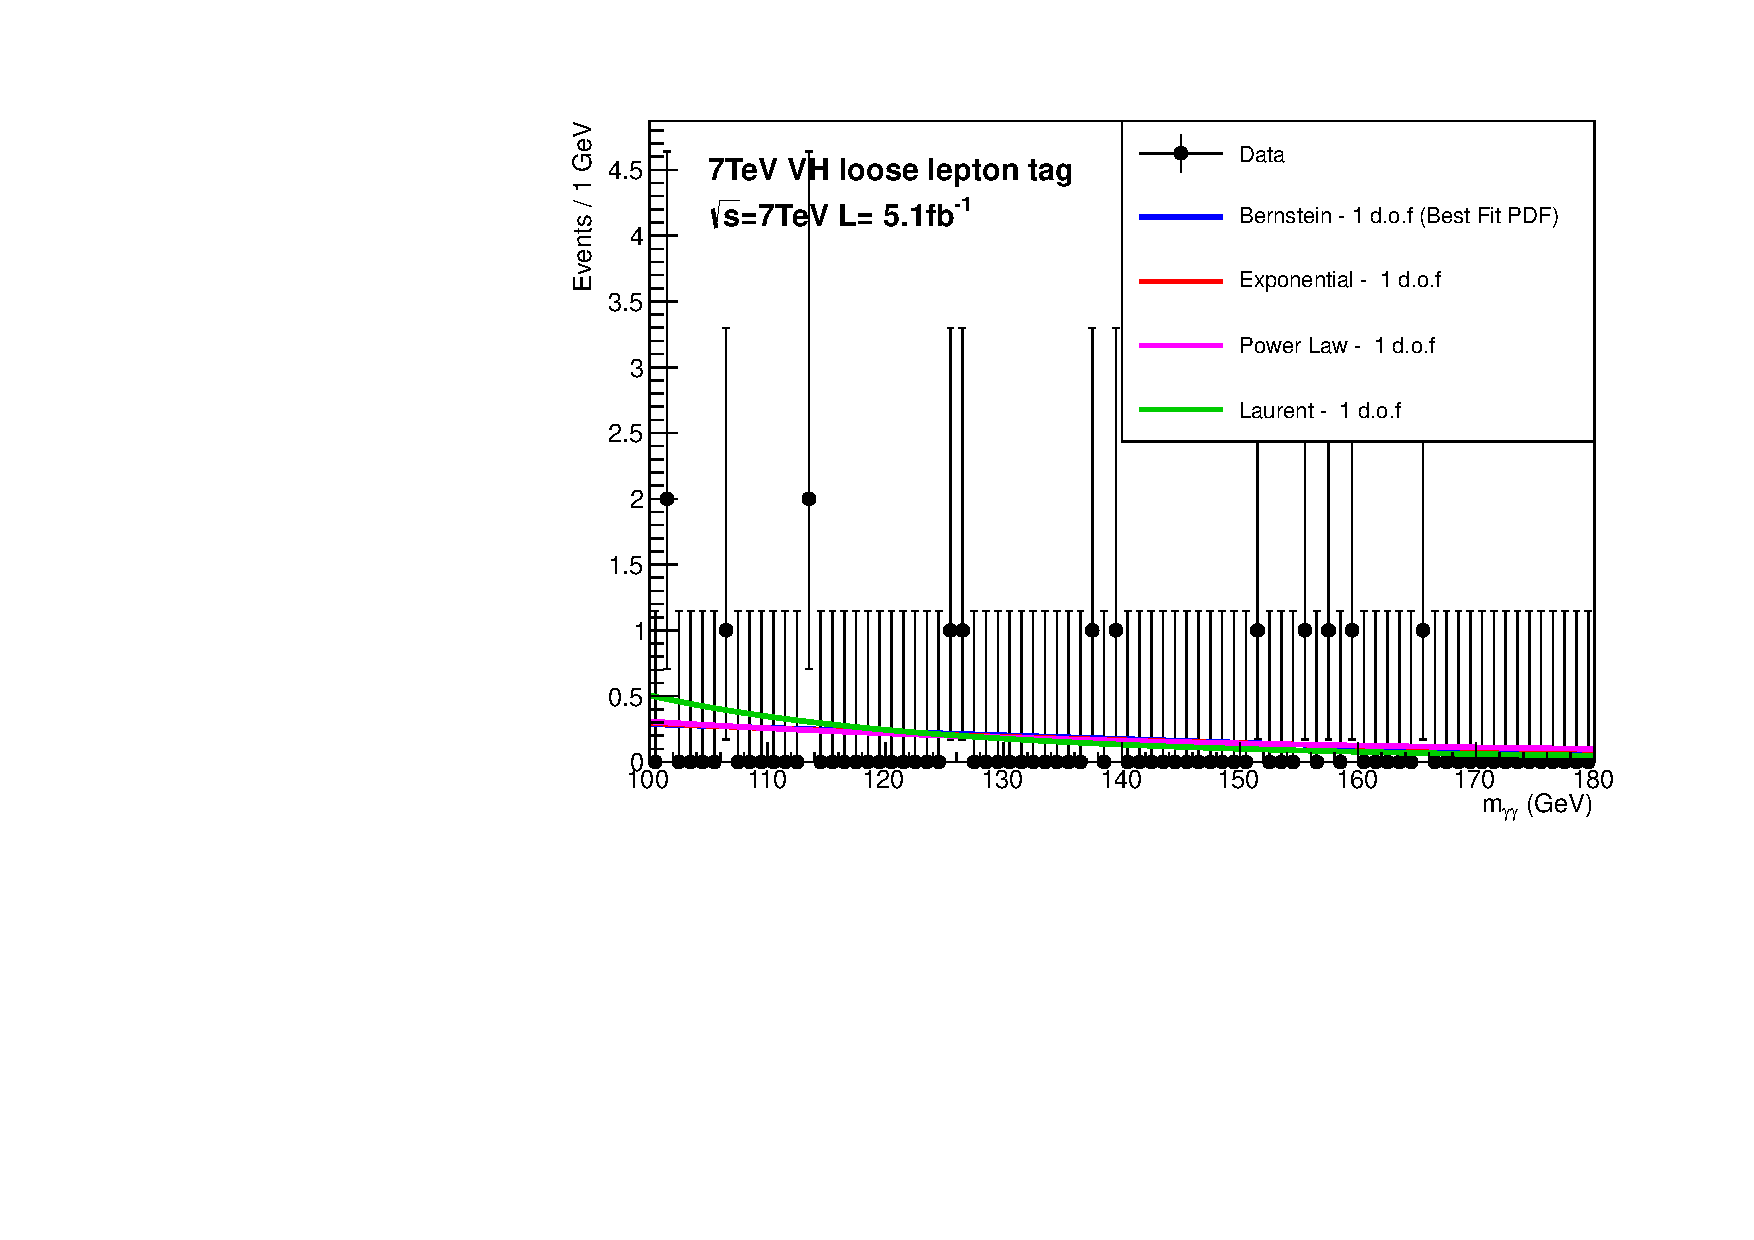
\includegraphics[width=0.49\textwidth]{analysis/plots/multipdf_plots/cat7_7TeV.pdf}
  \caption{The diphoton invariant mass distribution and the background function choices profiled using the envelope method for the inclusive, dijet and \VH lepton tag categories in the 7~\TeV dataset.}
  \label{fig:multipdf1}
\end{figure}

\begin{figure}
  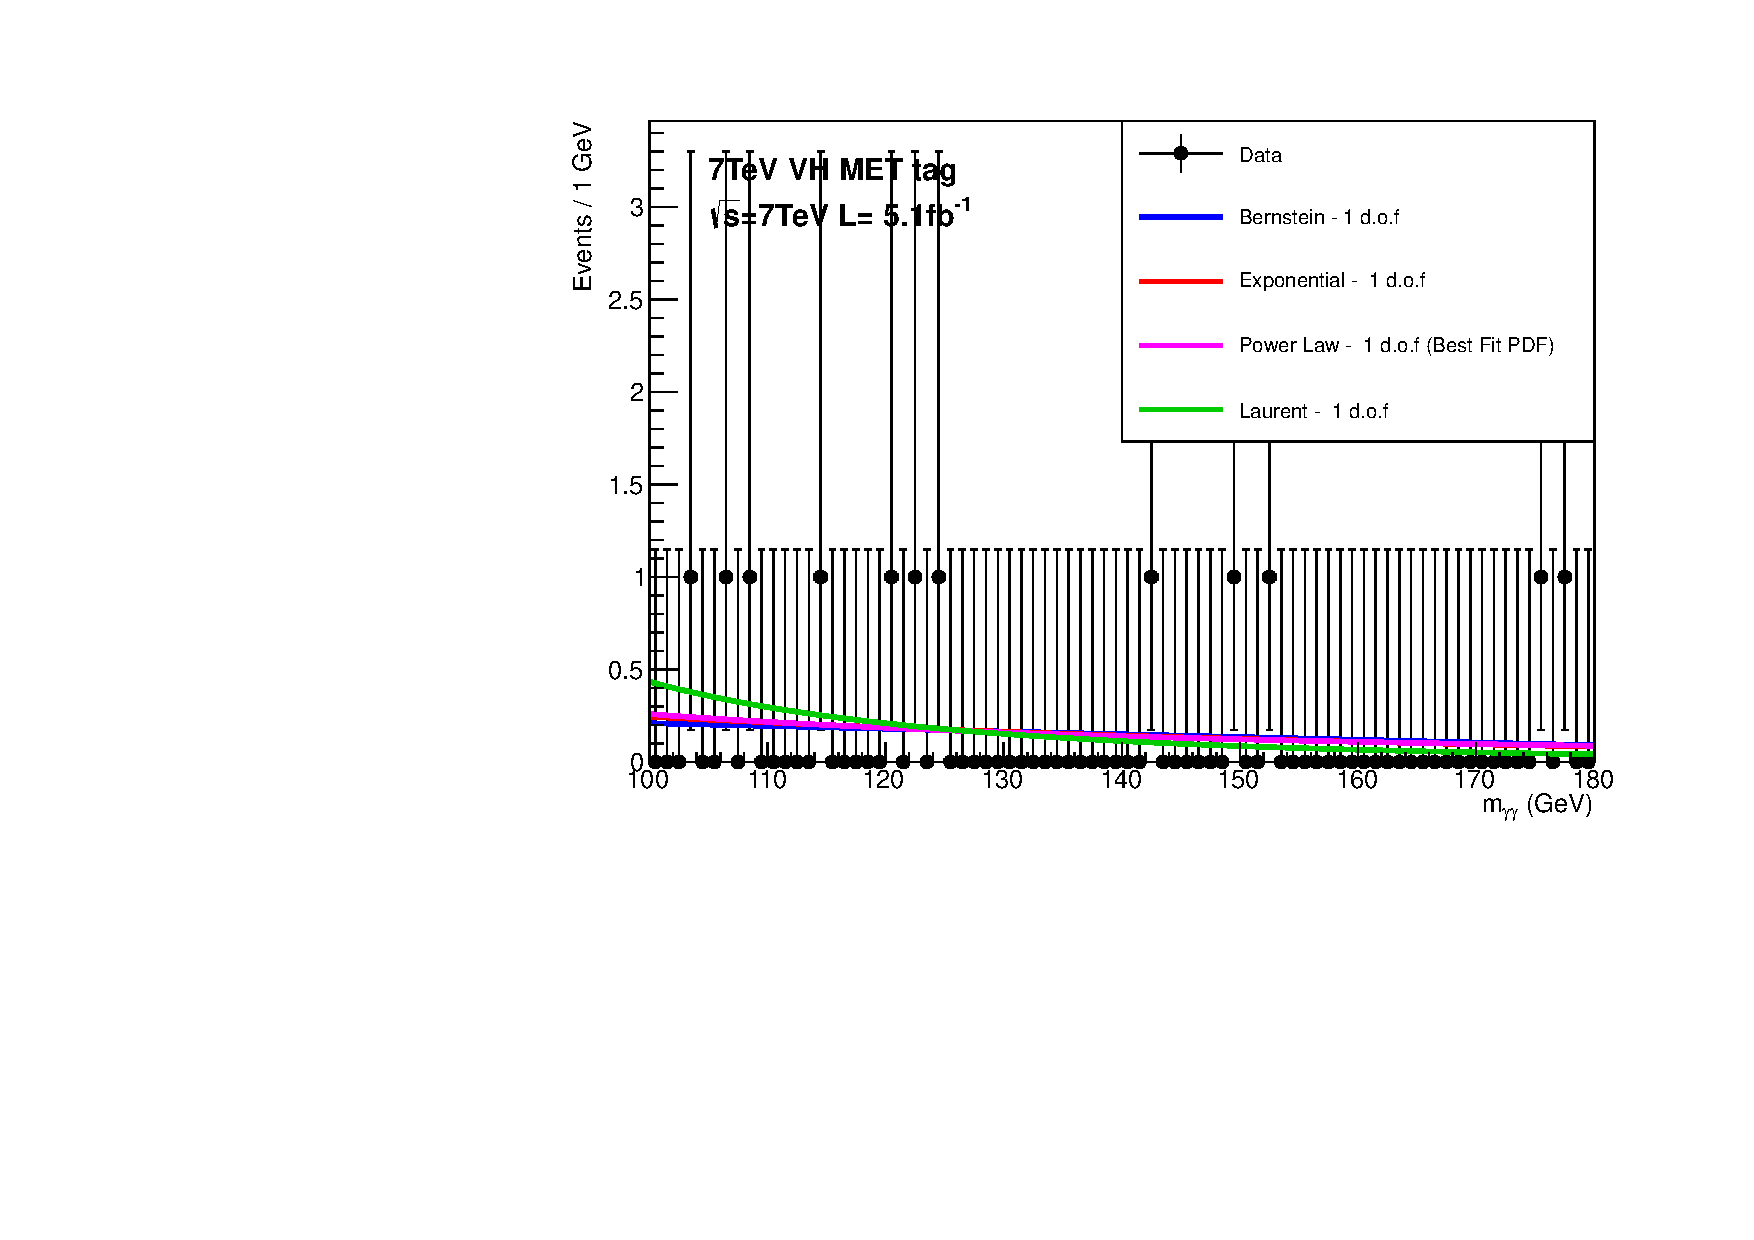
\includegraphics[width=0.49\textwidth]{analysis/plots/multipdf_plots/cat8_7TeV.pdf}
  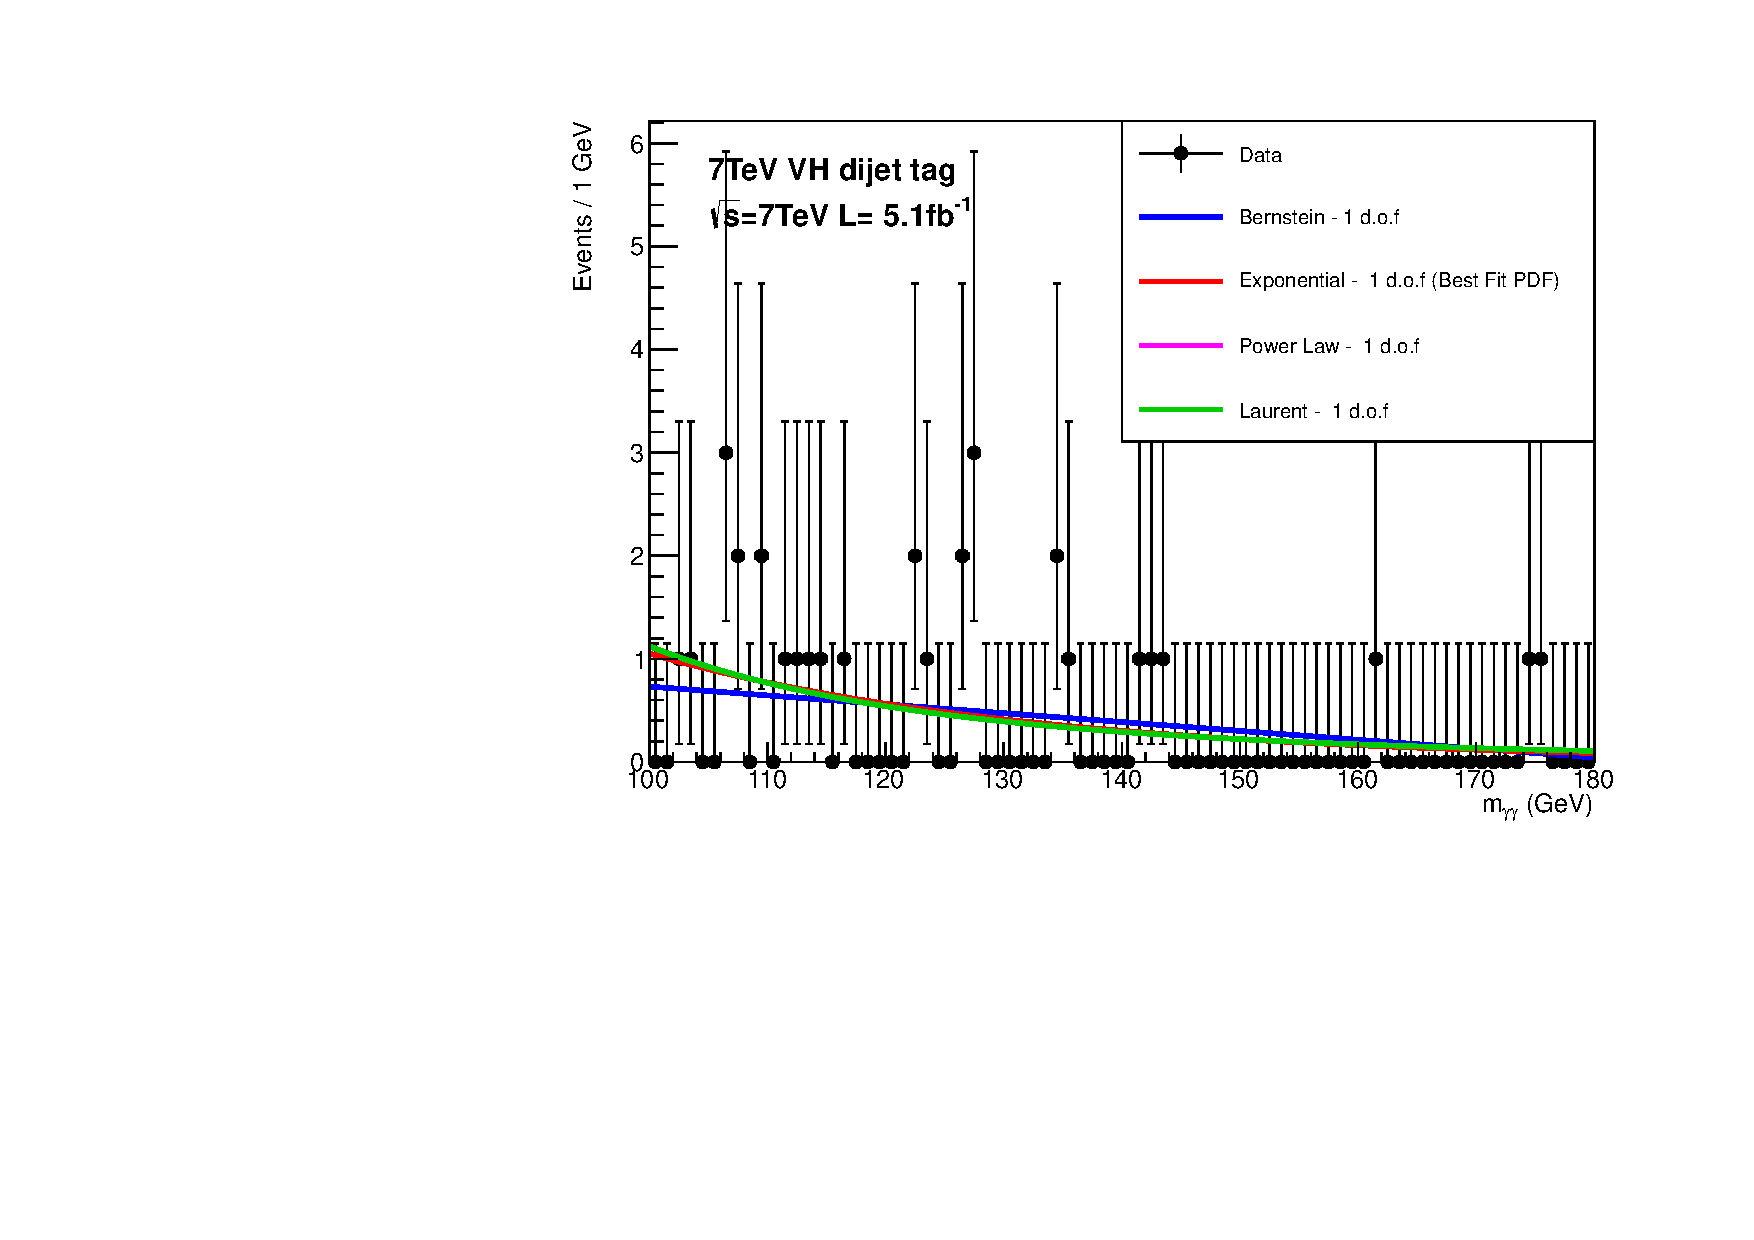
\includegraphics[width=0.49\textwidth]{analysis/plots/multipdf_plots/cat10_7TeV.pdf}\\
  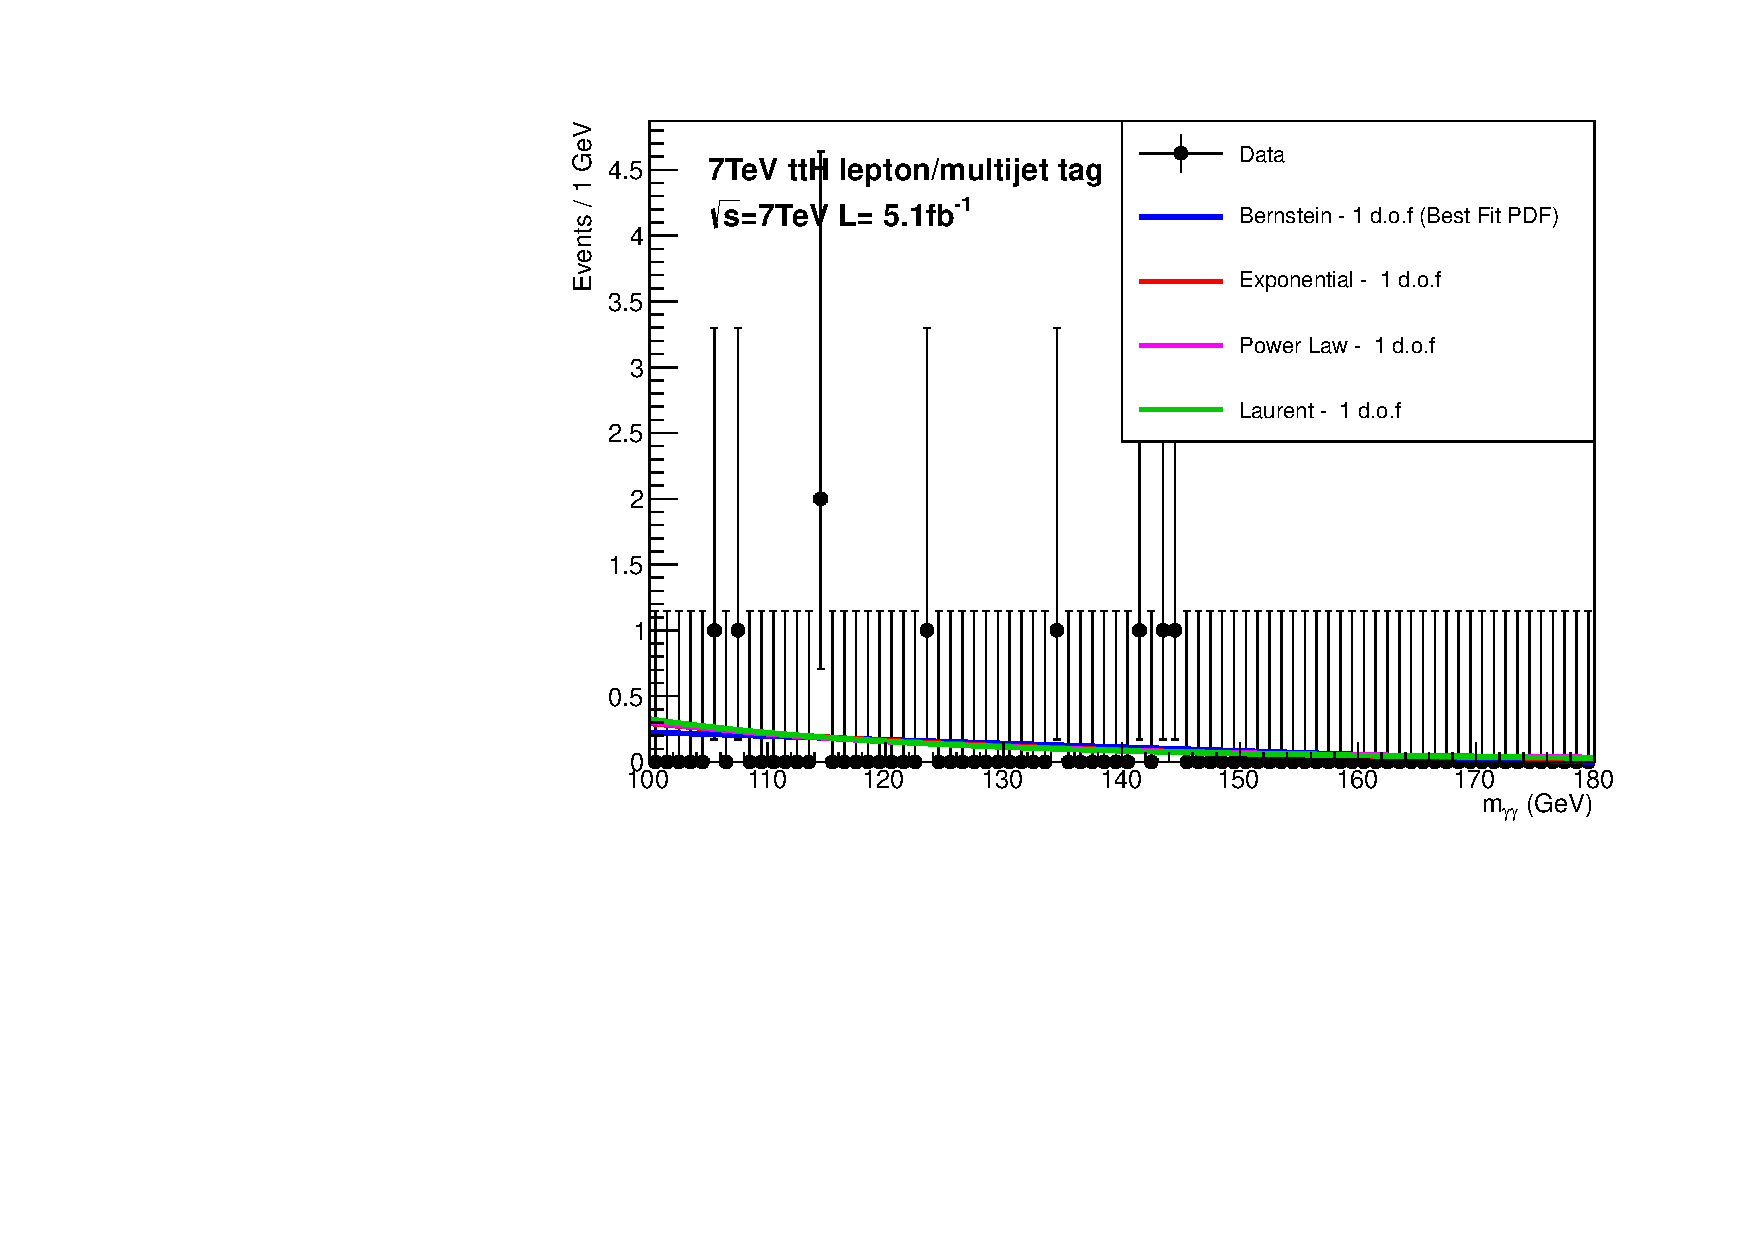
\includegraphics[width=0.49\textwidth]{analysis/plots/multipdf_plots/cat9_7TeV.pdf}
  \caption{The diphoton invariant mass distribution and the background function choices profiled using the envelope method for the \VH \MET and jet tag and \ttH categories in the 7~\TeV dataset.}
  \label{fig:multipdf2}
\end{figure}

\begin{figure}
  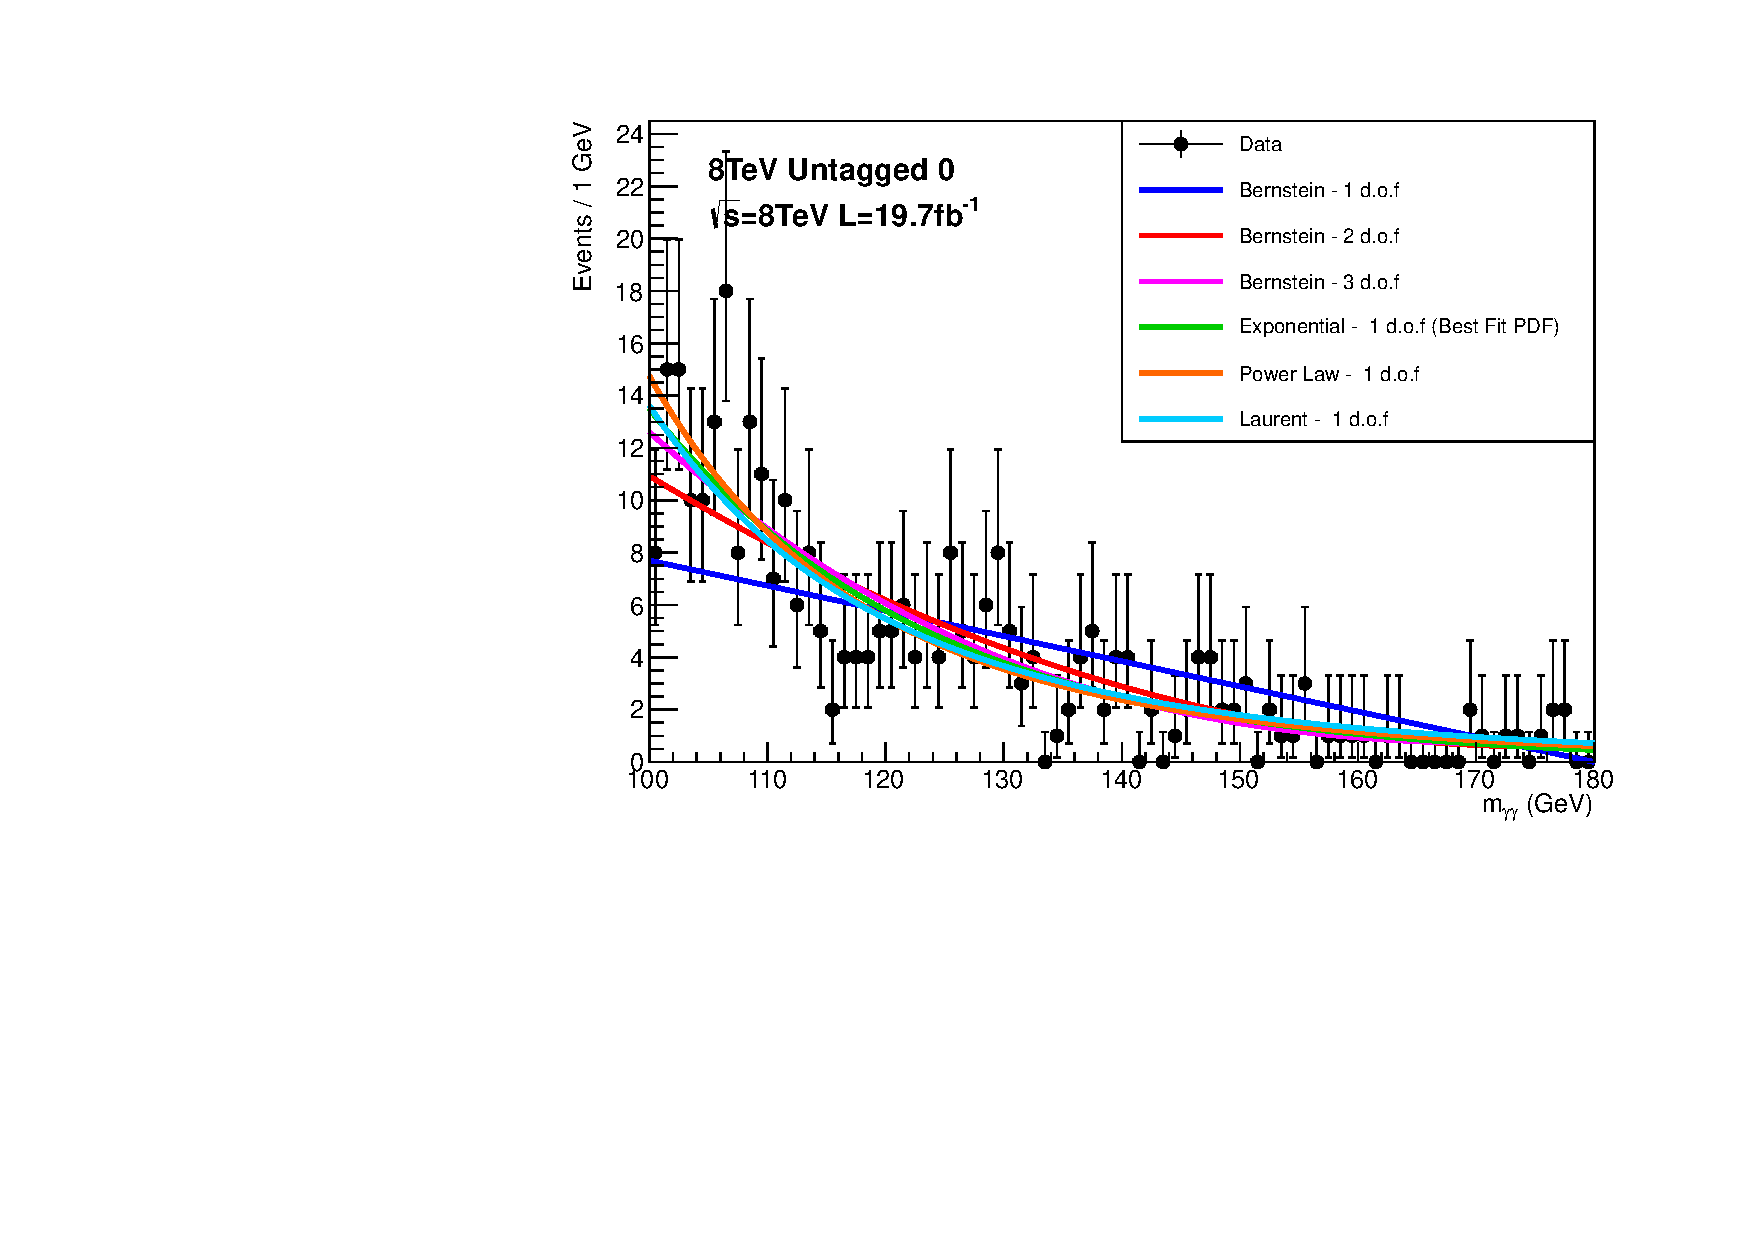
\includegraphics[width=0.49\textwidth]{analysis/plots/multipdf_plots/cat0_8TeV.pdf}
  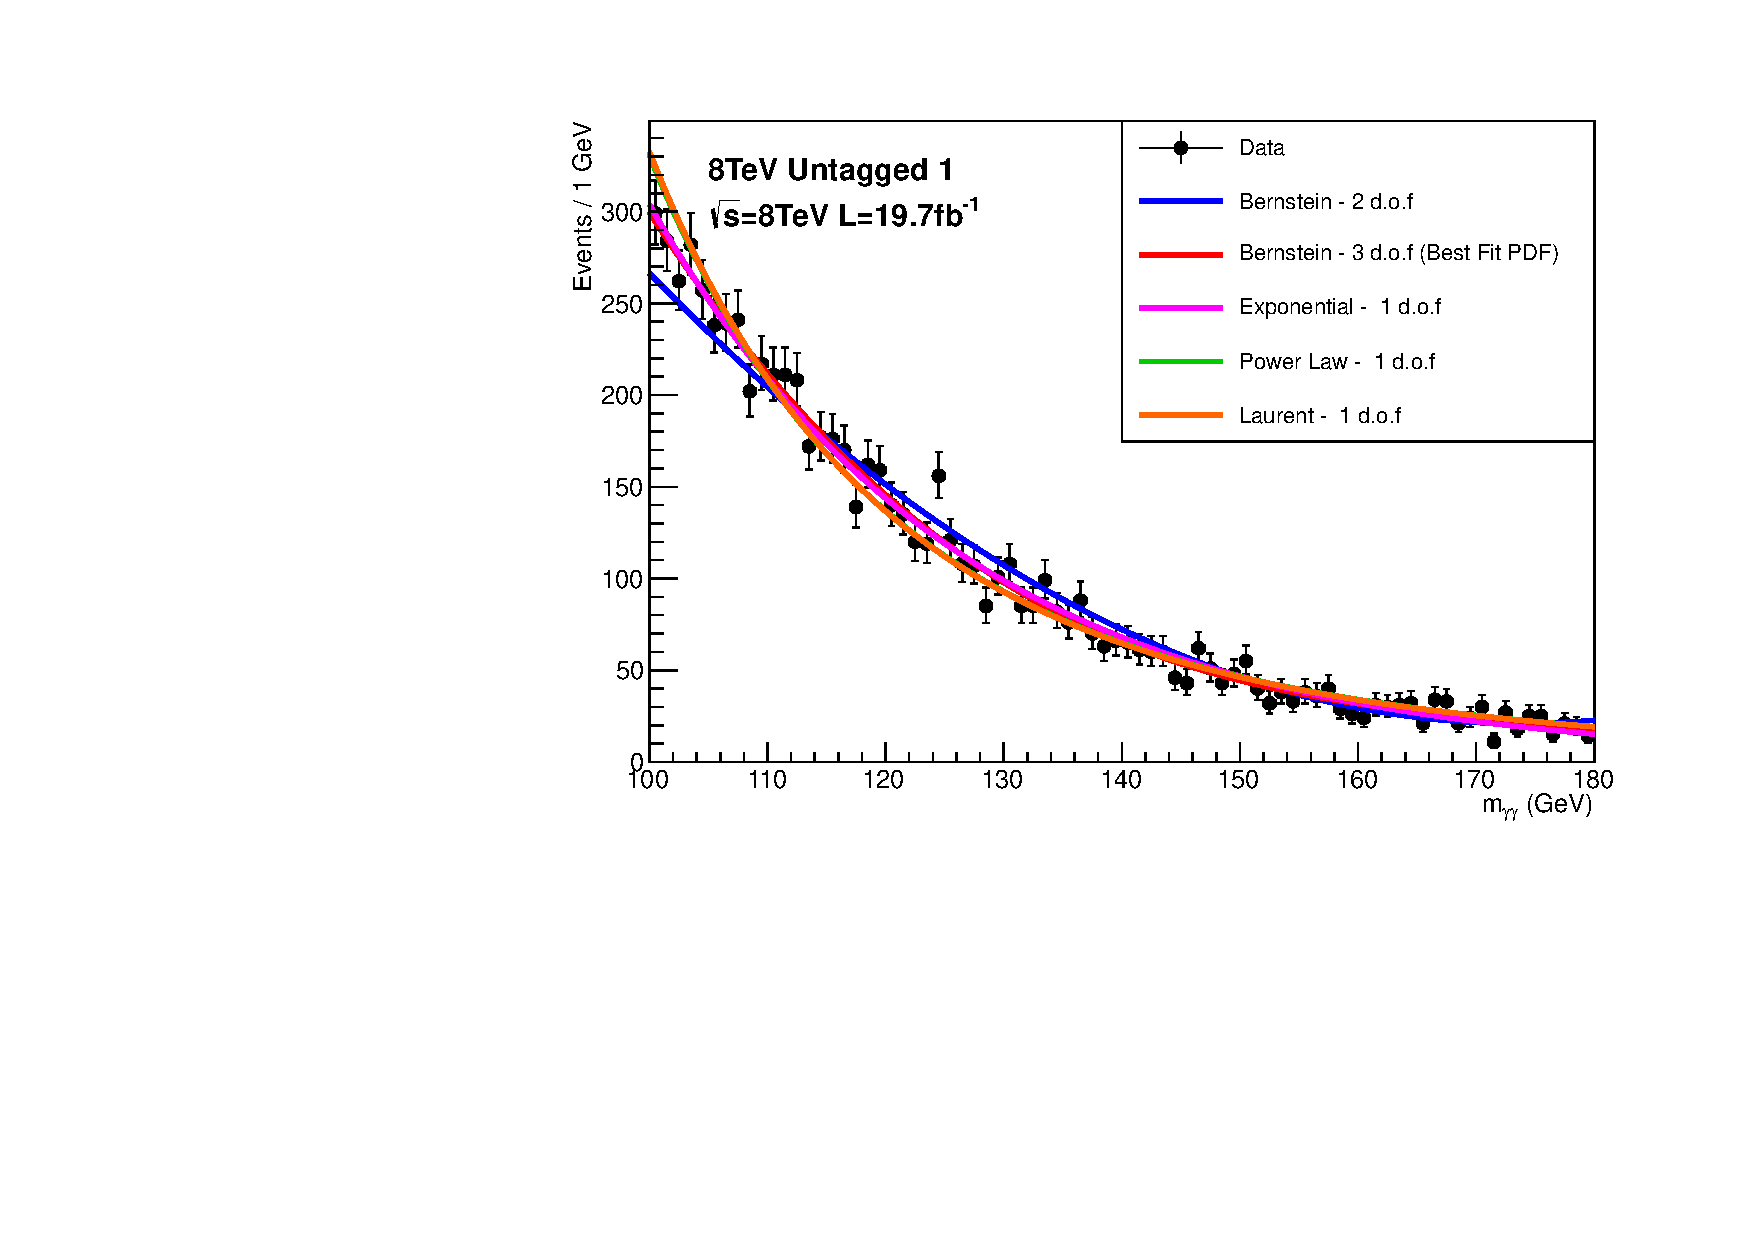
\includegraphics[width=0.49\textwidth]{analysis/plots/multipdf_plots/cat1_8TeV.pdf}\\
  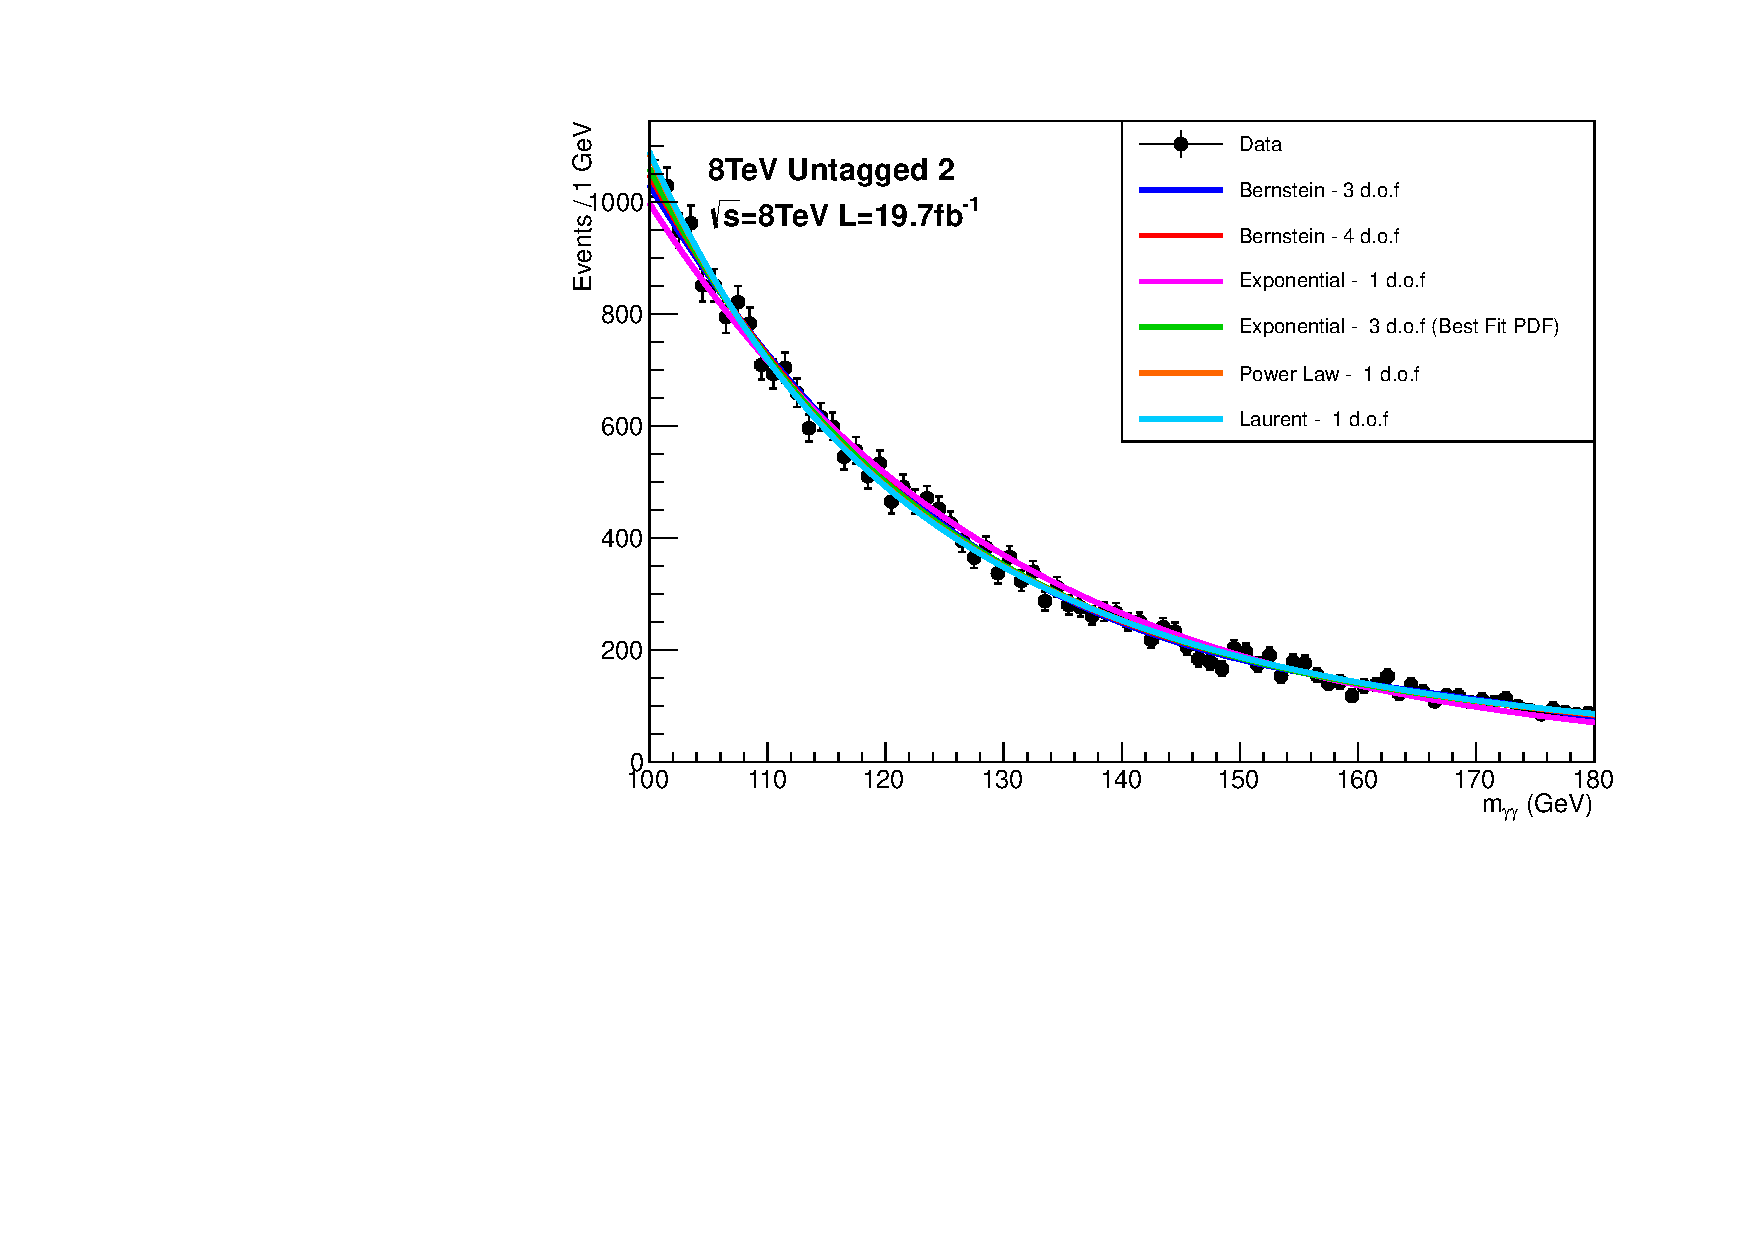
\includegraphics[width=0.49\textwidth]{analysis/plots/multipdf_plots/cat2_8TeV.pdf}
  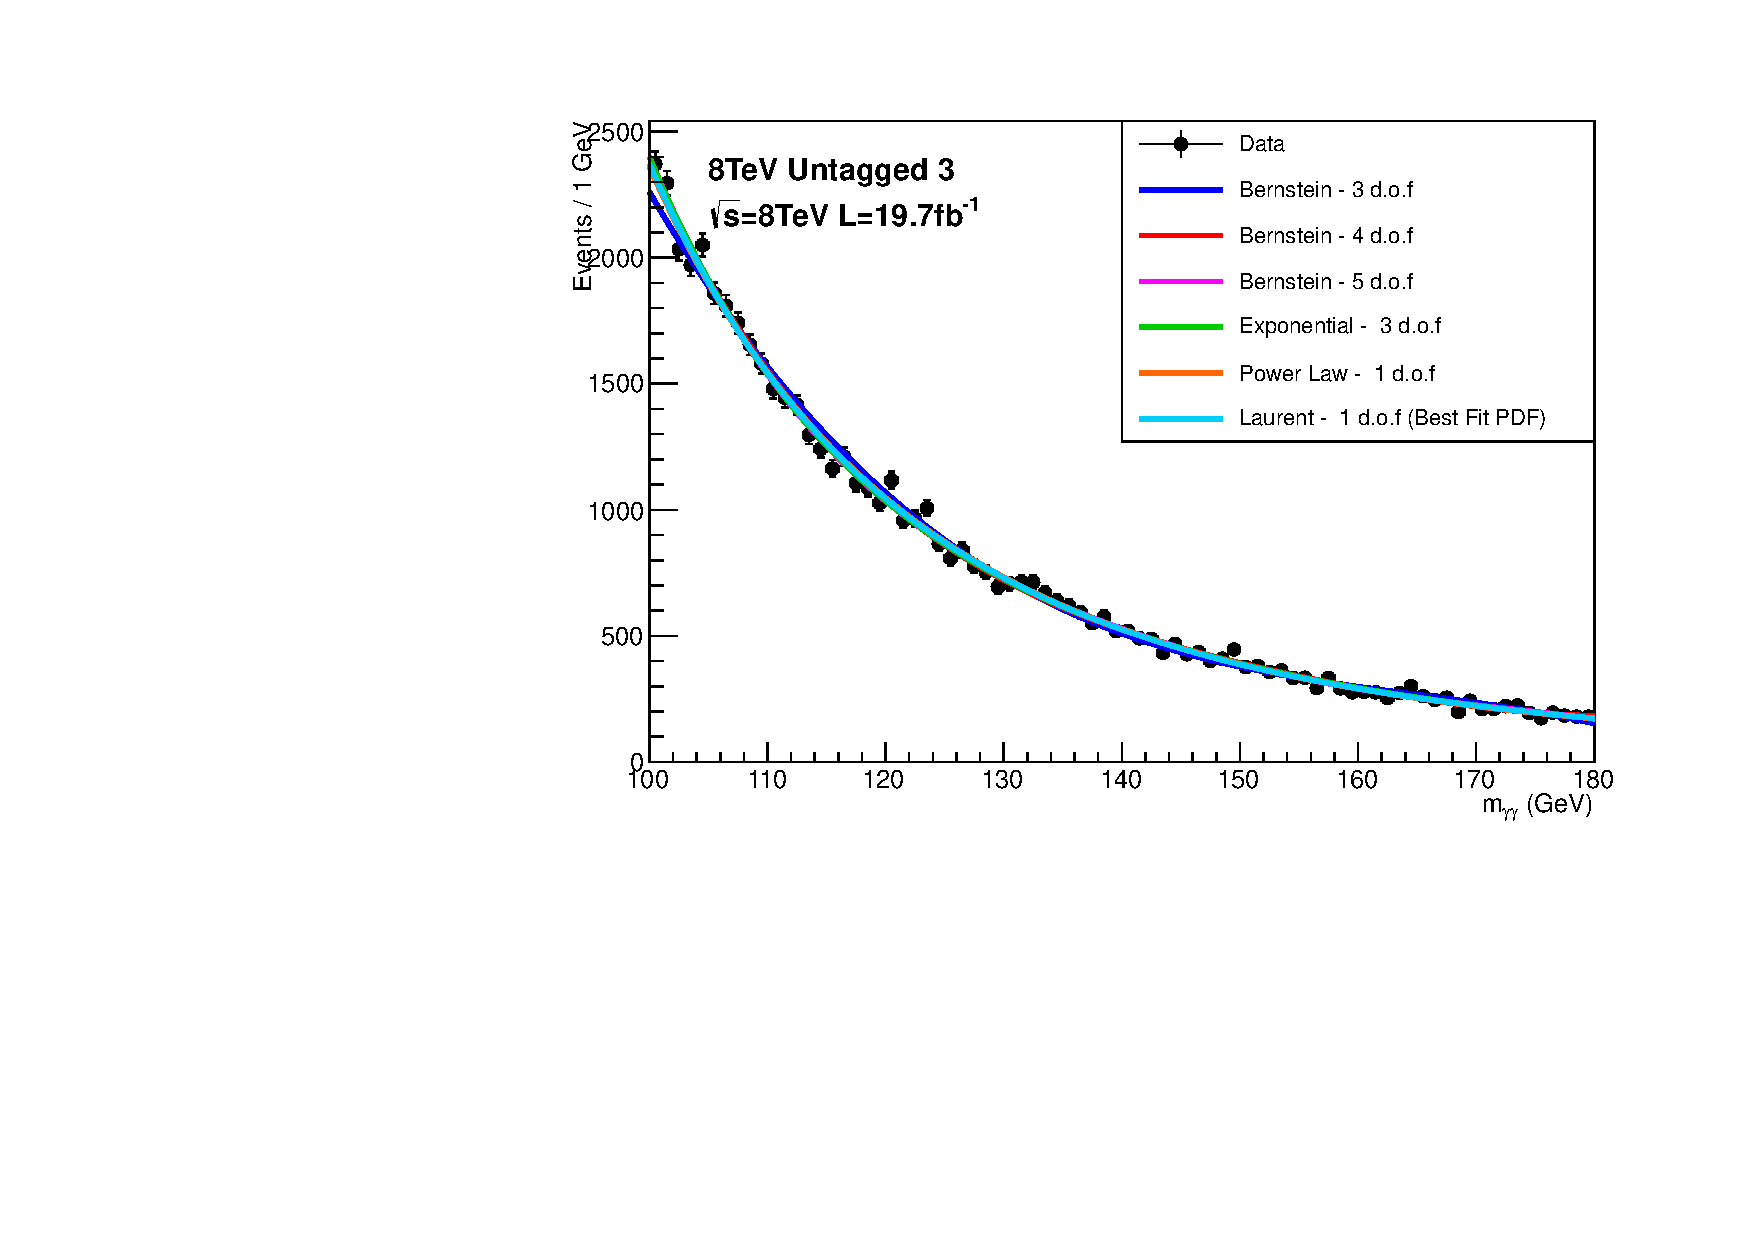
\includegraphics[width=0.49\textwidth]{analysis/plots/multipdf_plots/cat3_8TeV.pdf}\\
  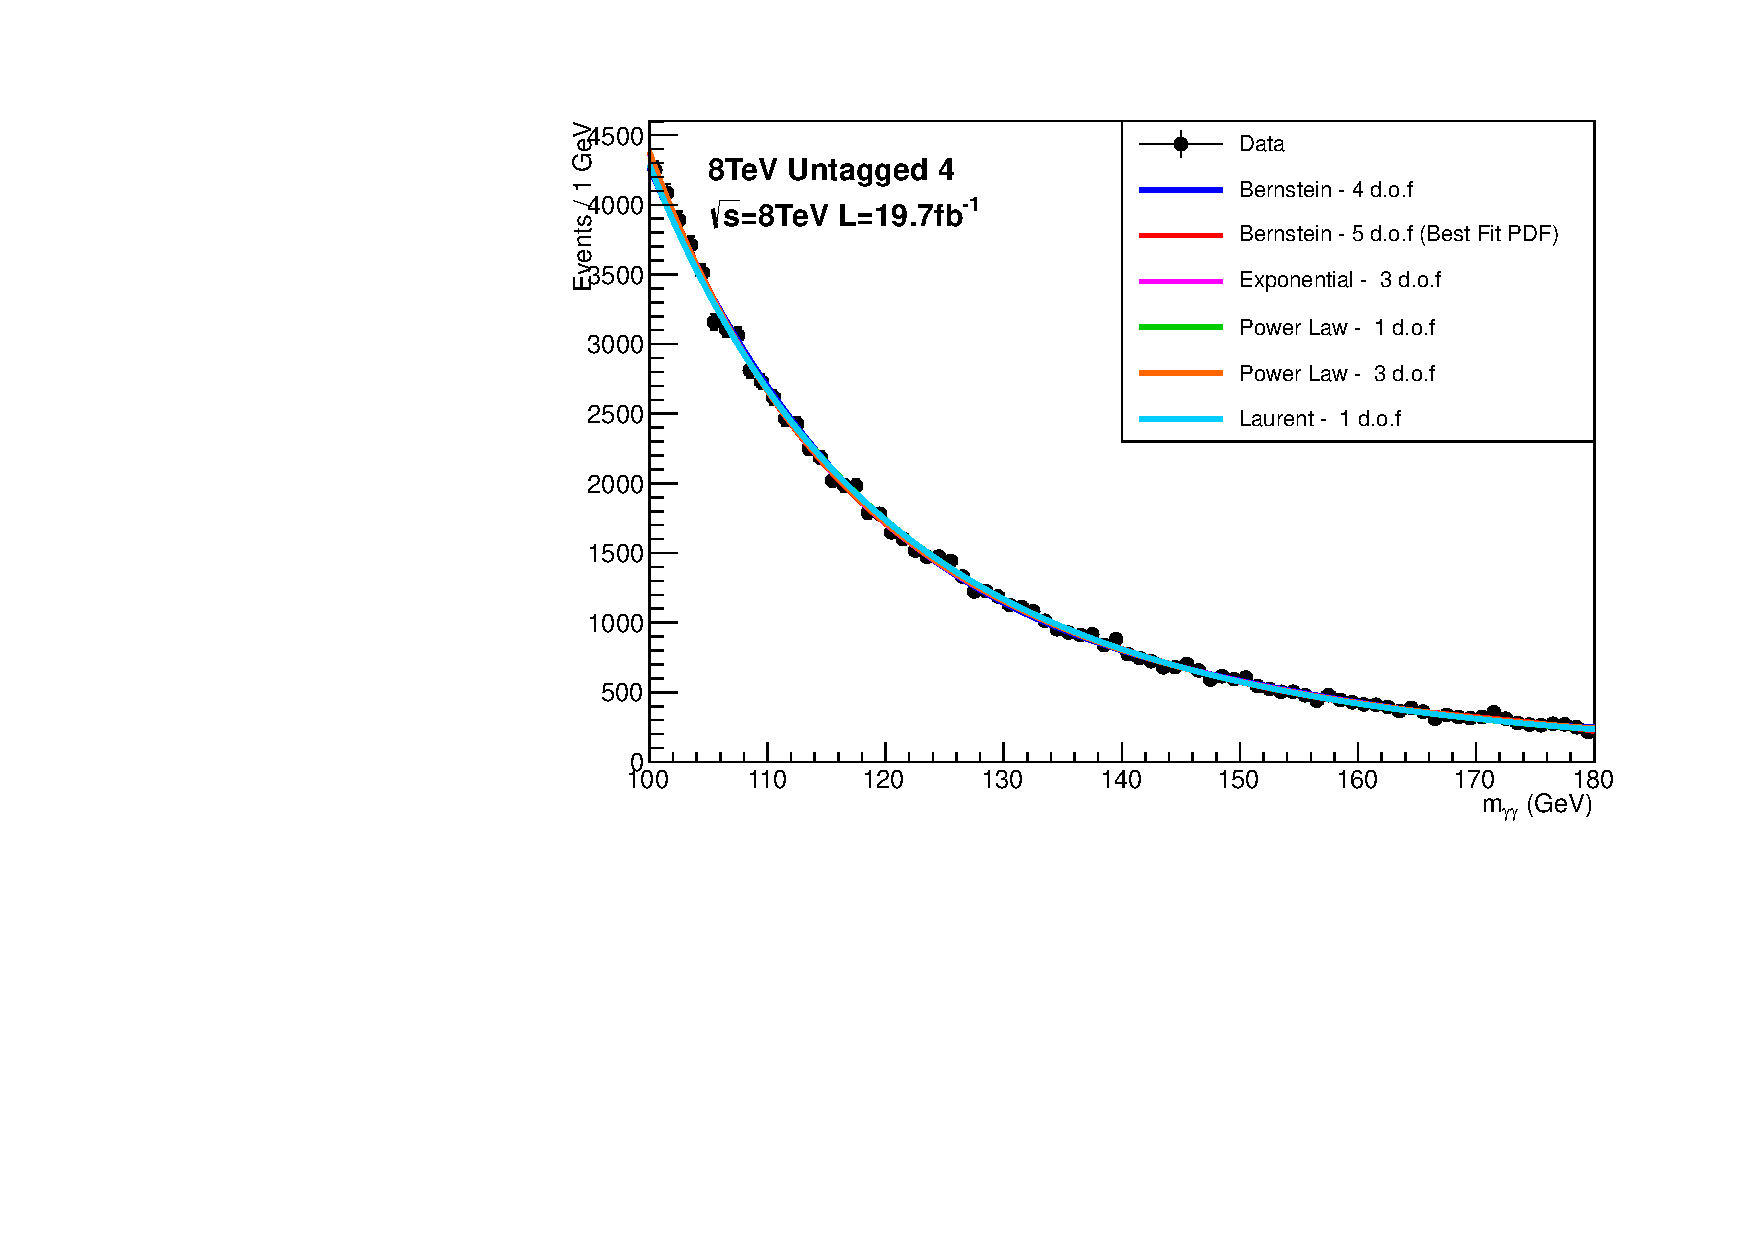
\includegraphics[width=0.49\textwidth]{analysis/plots/multipdf_plots/cat4_8TeV.pdf}
  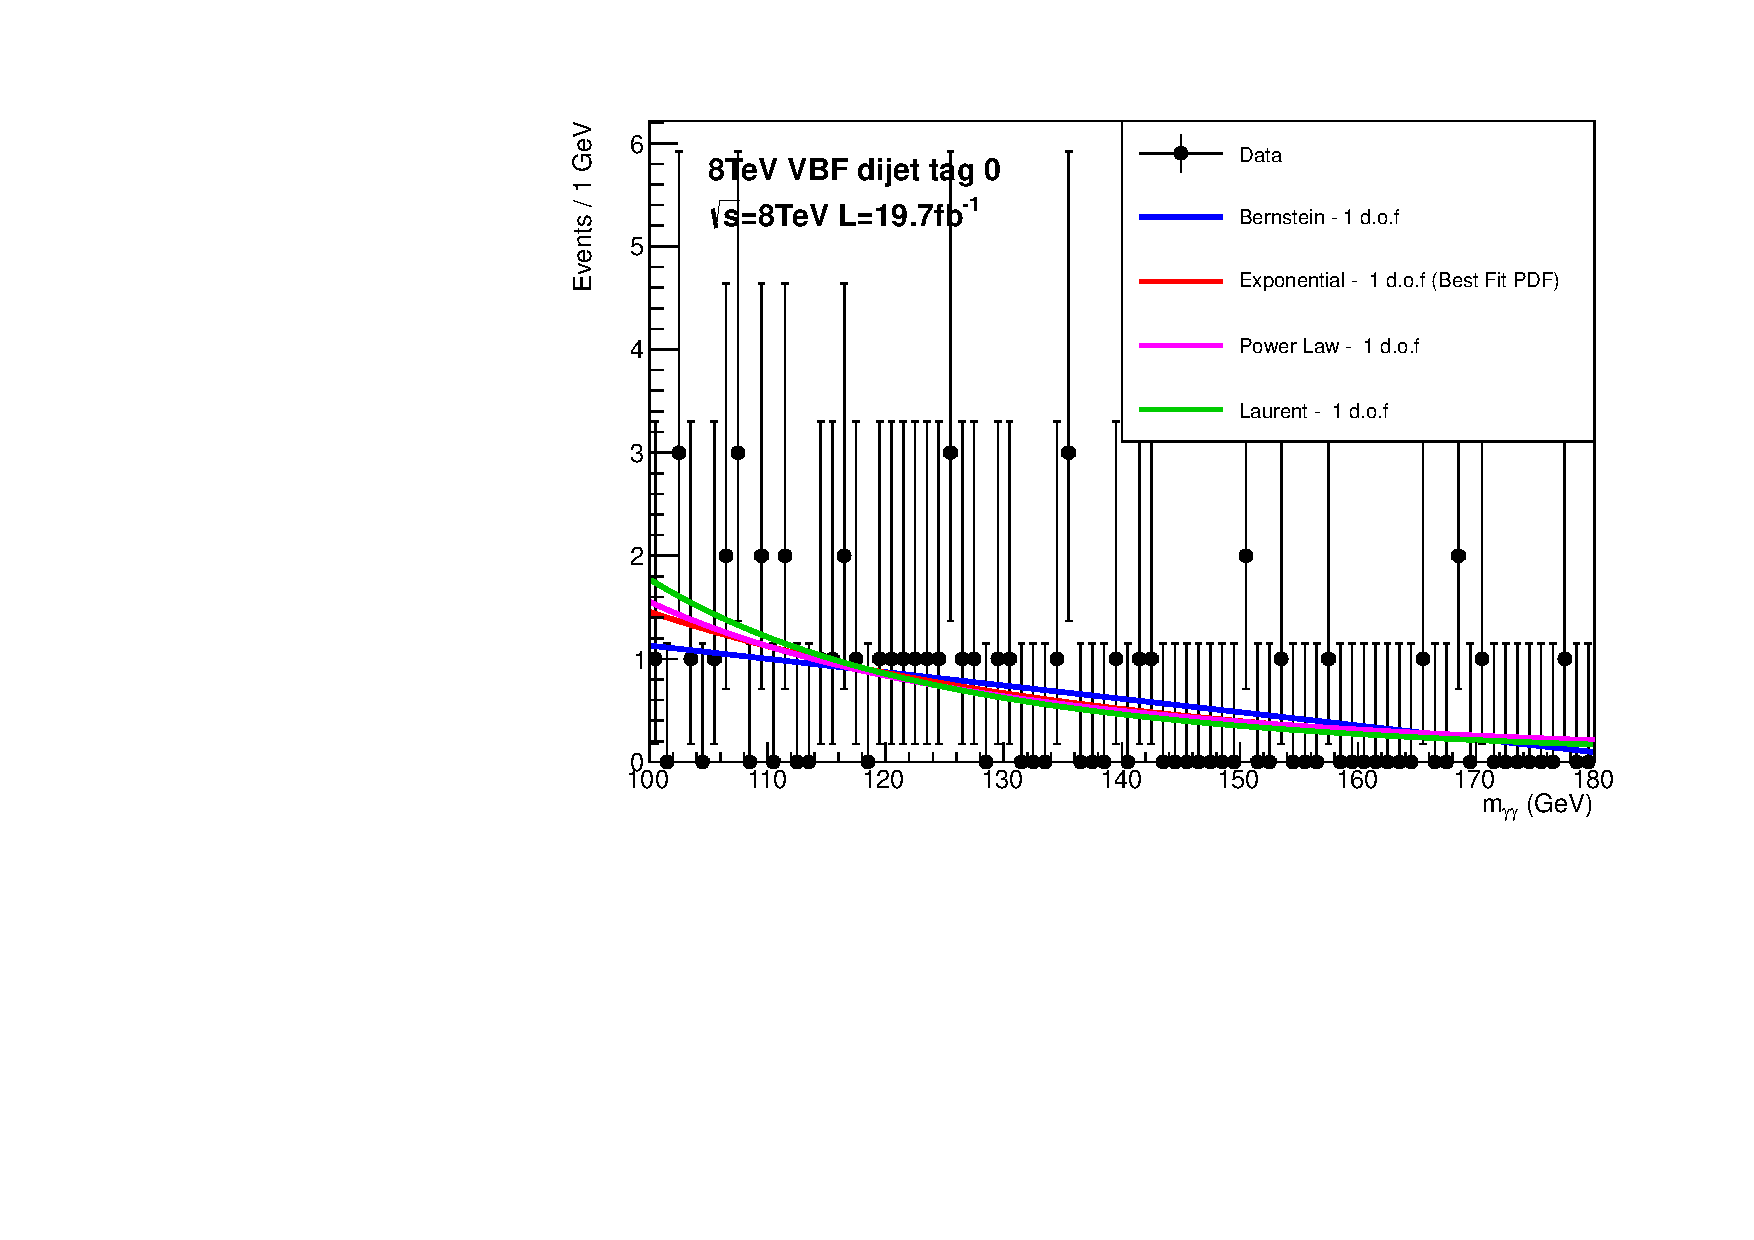
\includegraphics[width=0.49\textwidth]{analysis/plots/multipdf_plots/cat5_8TeV.pdf}\\
  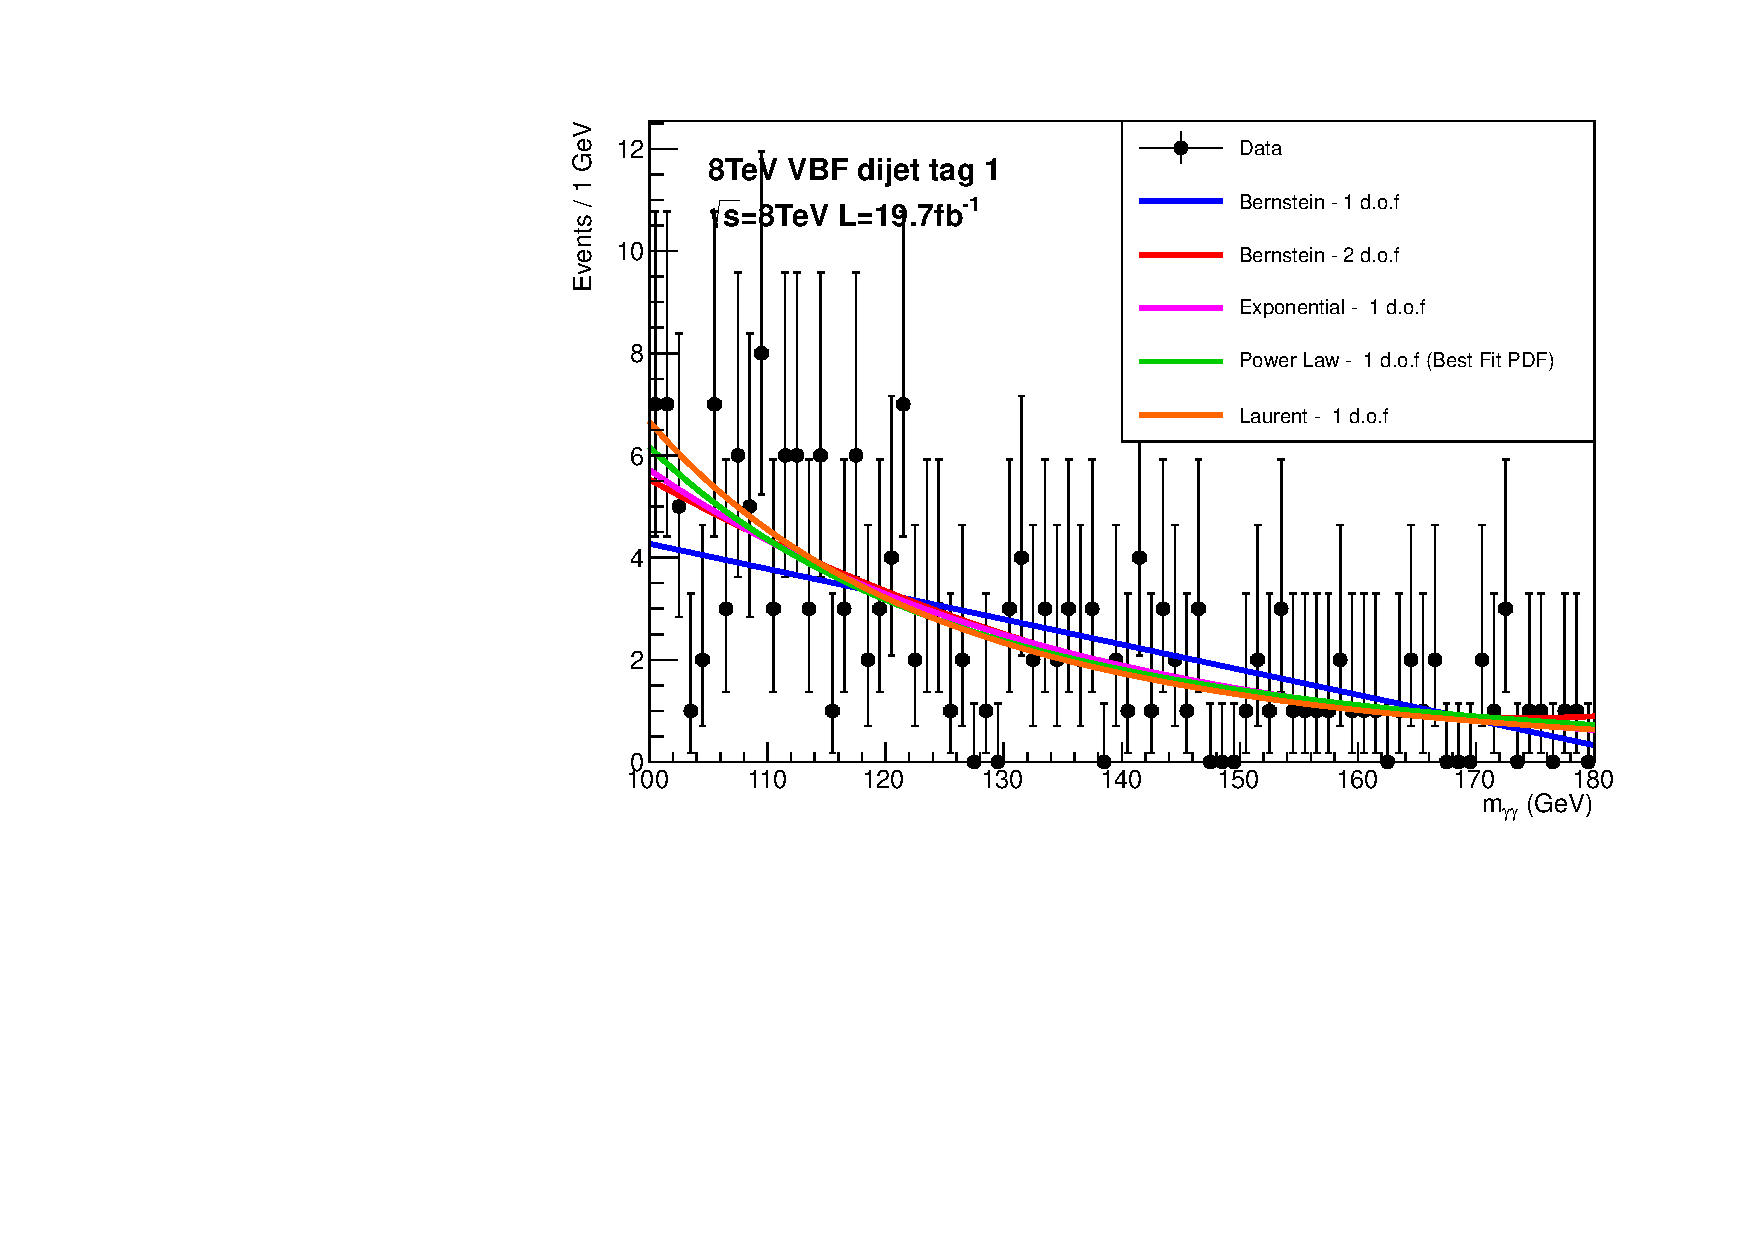
\includegraphics[width=0.49\textwidth]{analysis/plots/multipdf_plots/cat6_8TeV.pdf}
  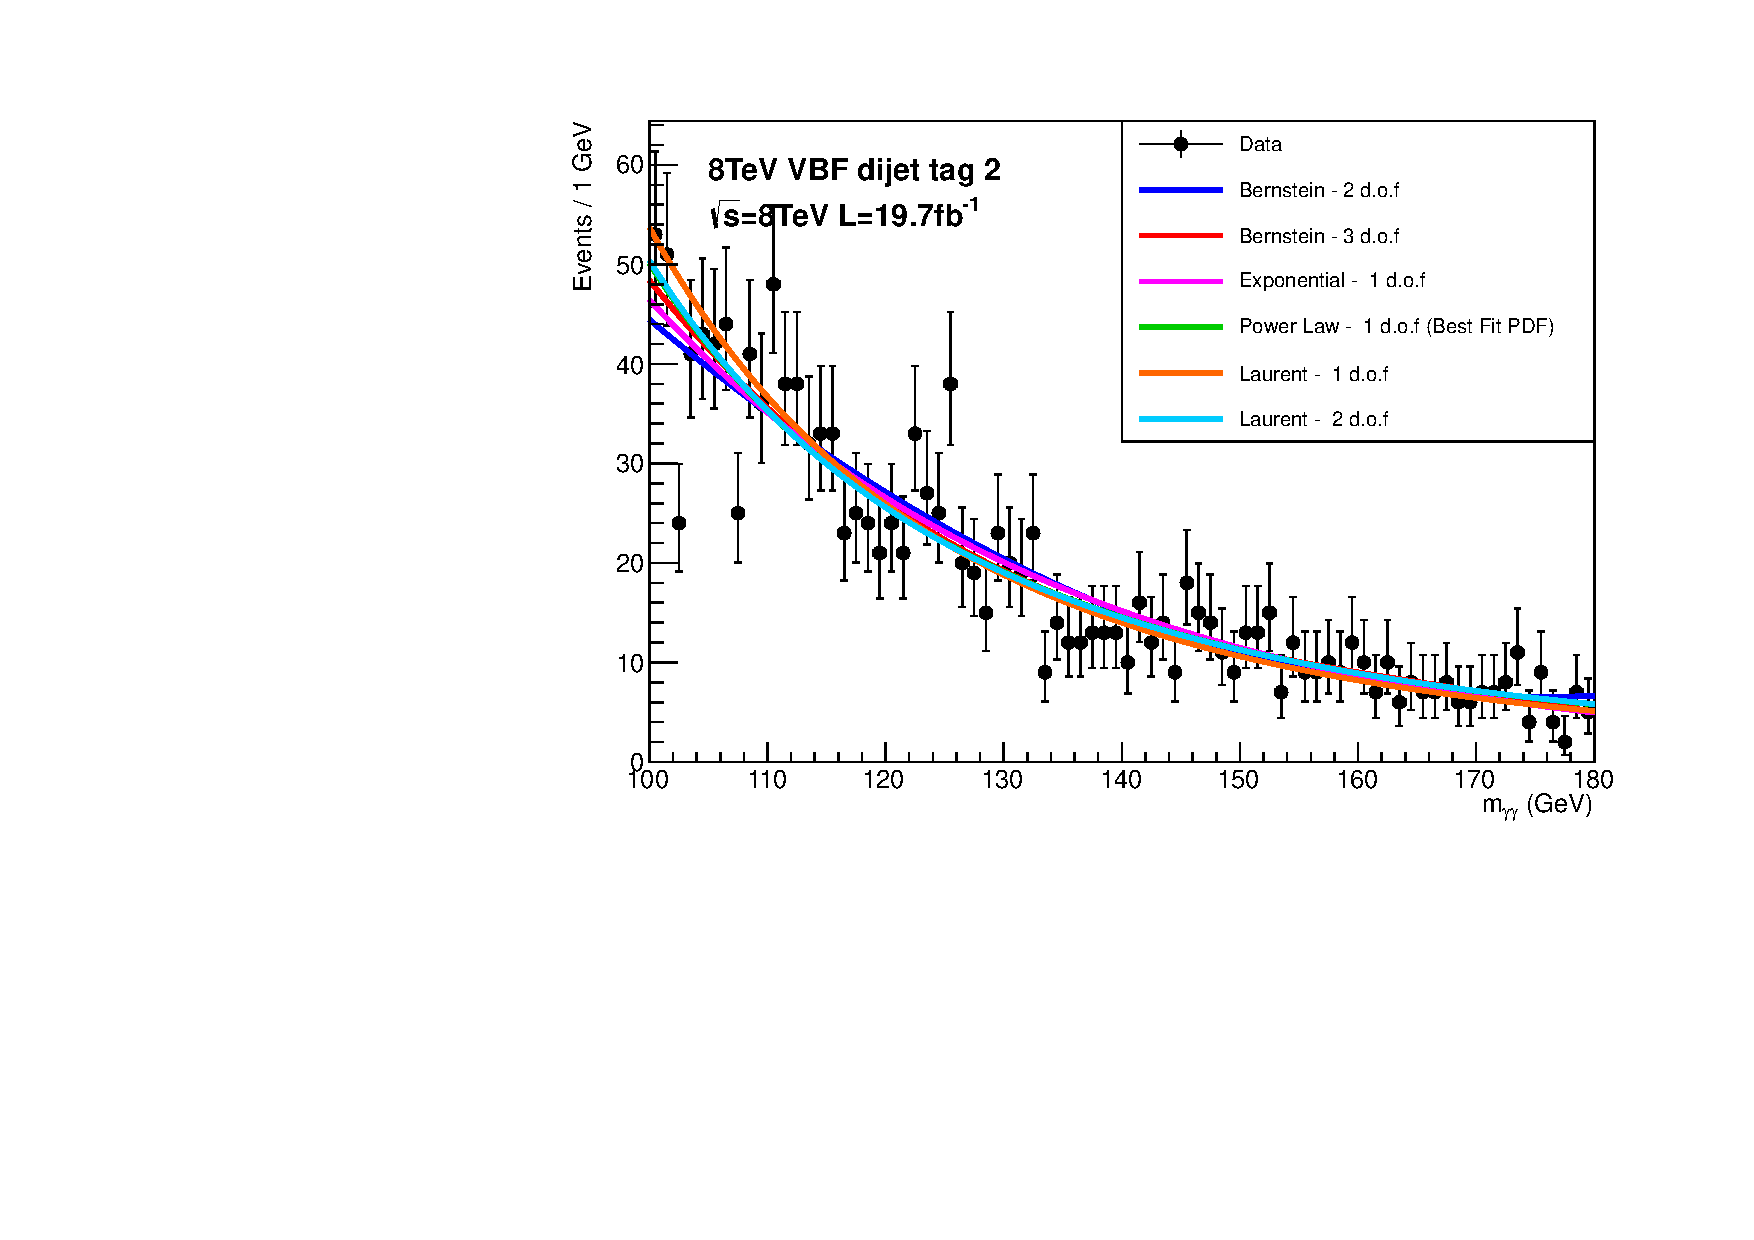
\includegraphics[width=0.49\textwidth]{analysis/plots/multipdf_plots/cat7_8TeV.pdf}
  \caption{The diphoton invariant mass distribution and the background function choices profiled using the envelope method for the inclusive and \VBF dijet tag categories in the 8~\TeV dataset.}
  \label{fig:multipdf3}
\end{figure}

\begin{figure}
  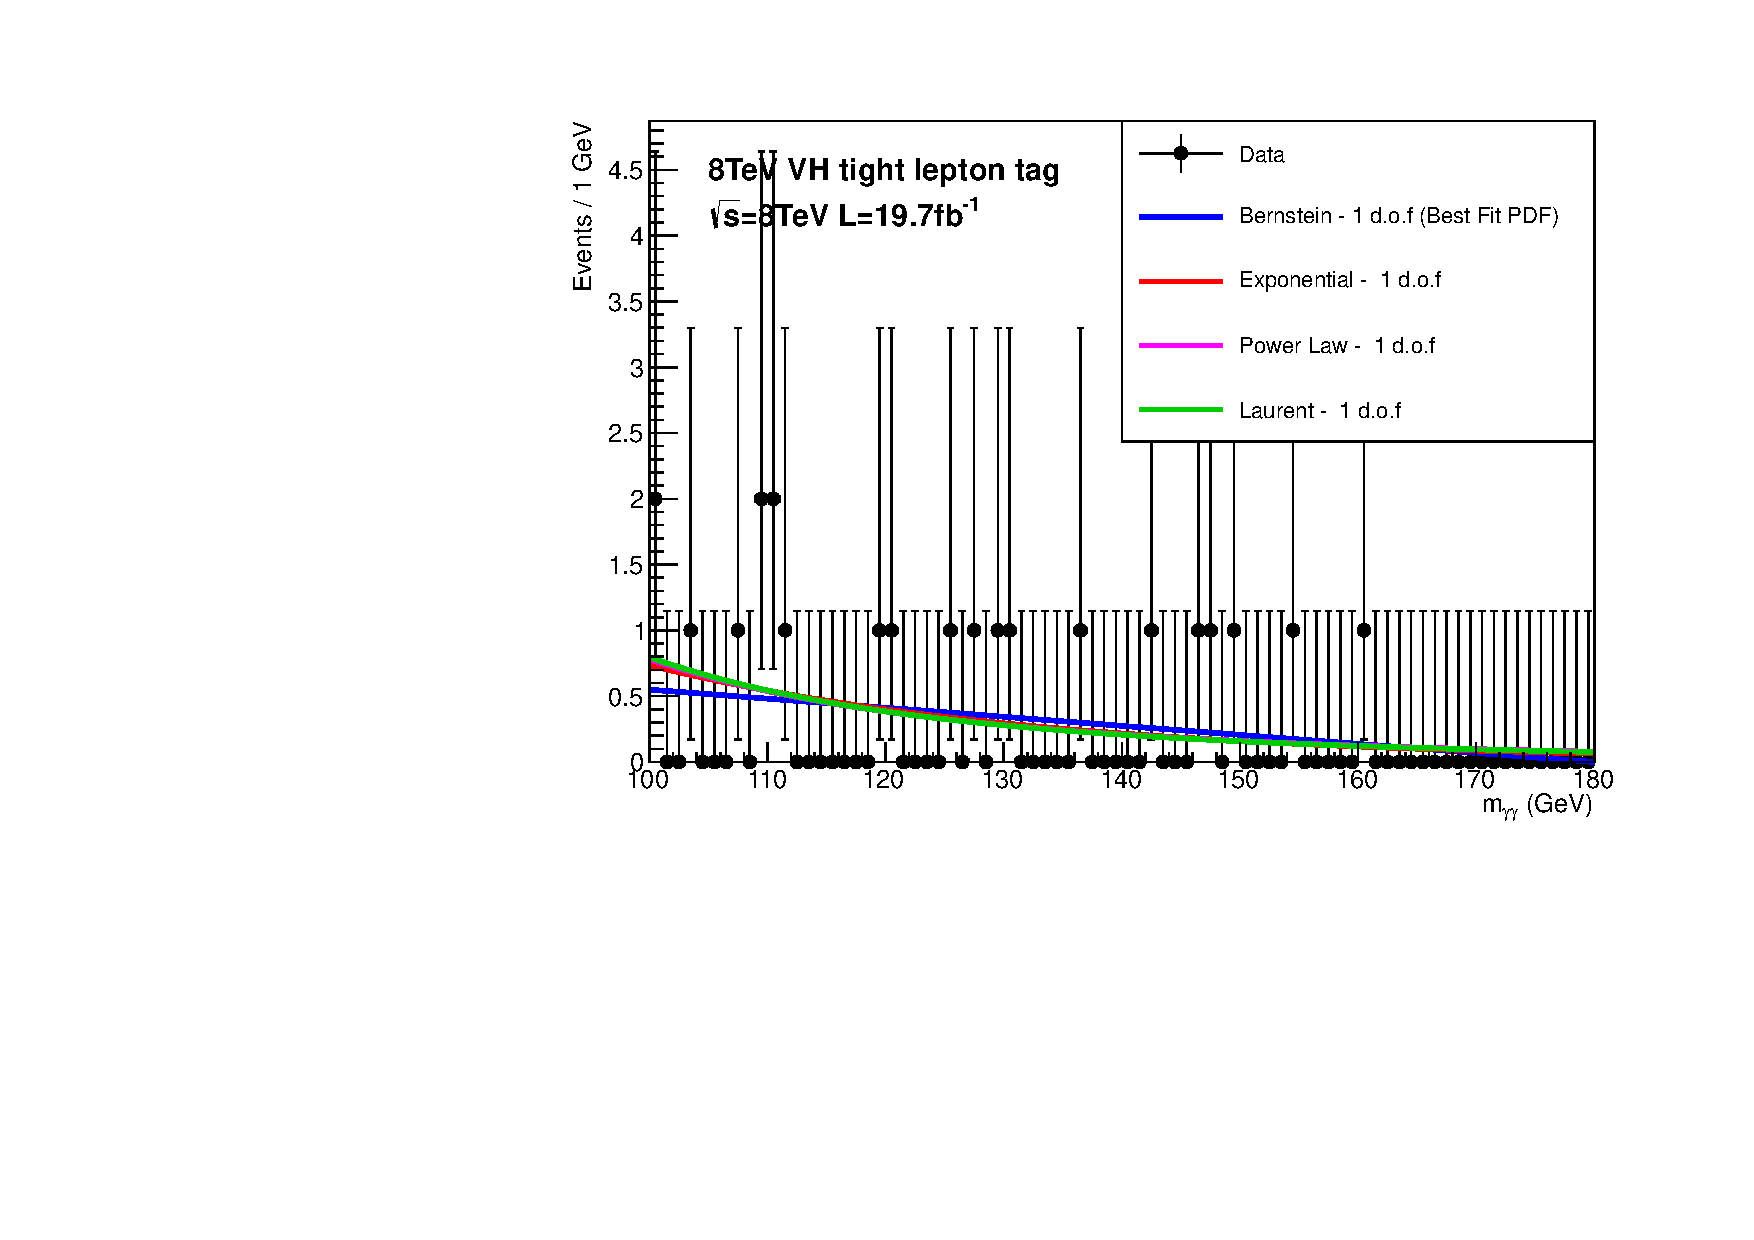
\includegraphics[width=0.49\textwidth]{analysis/plots/multipdf_plots/cat8_8TeV.pdf}
  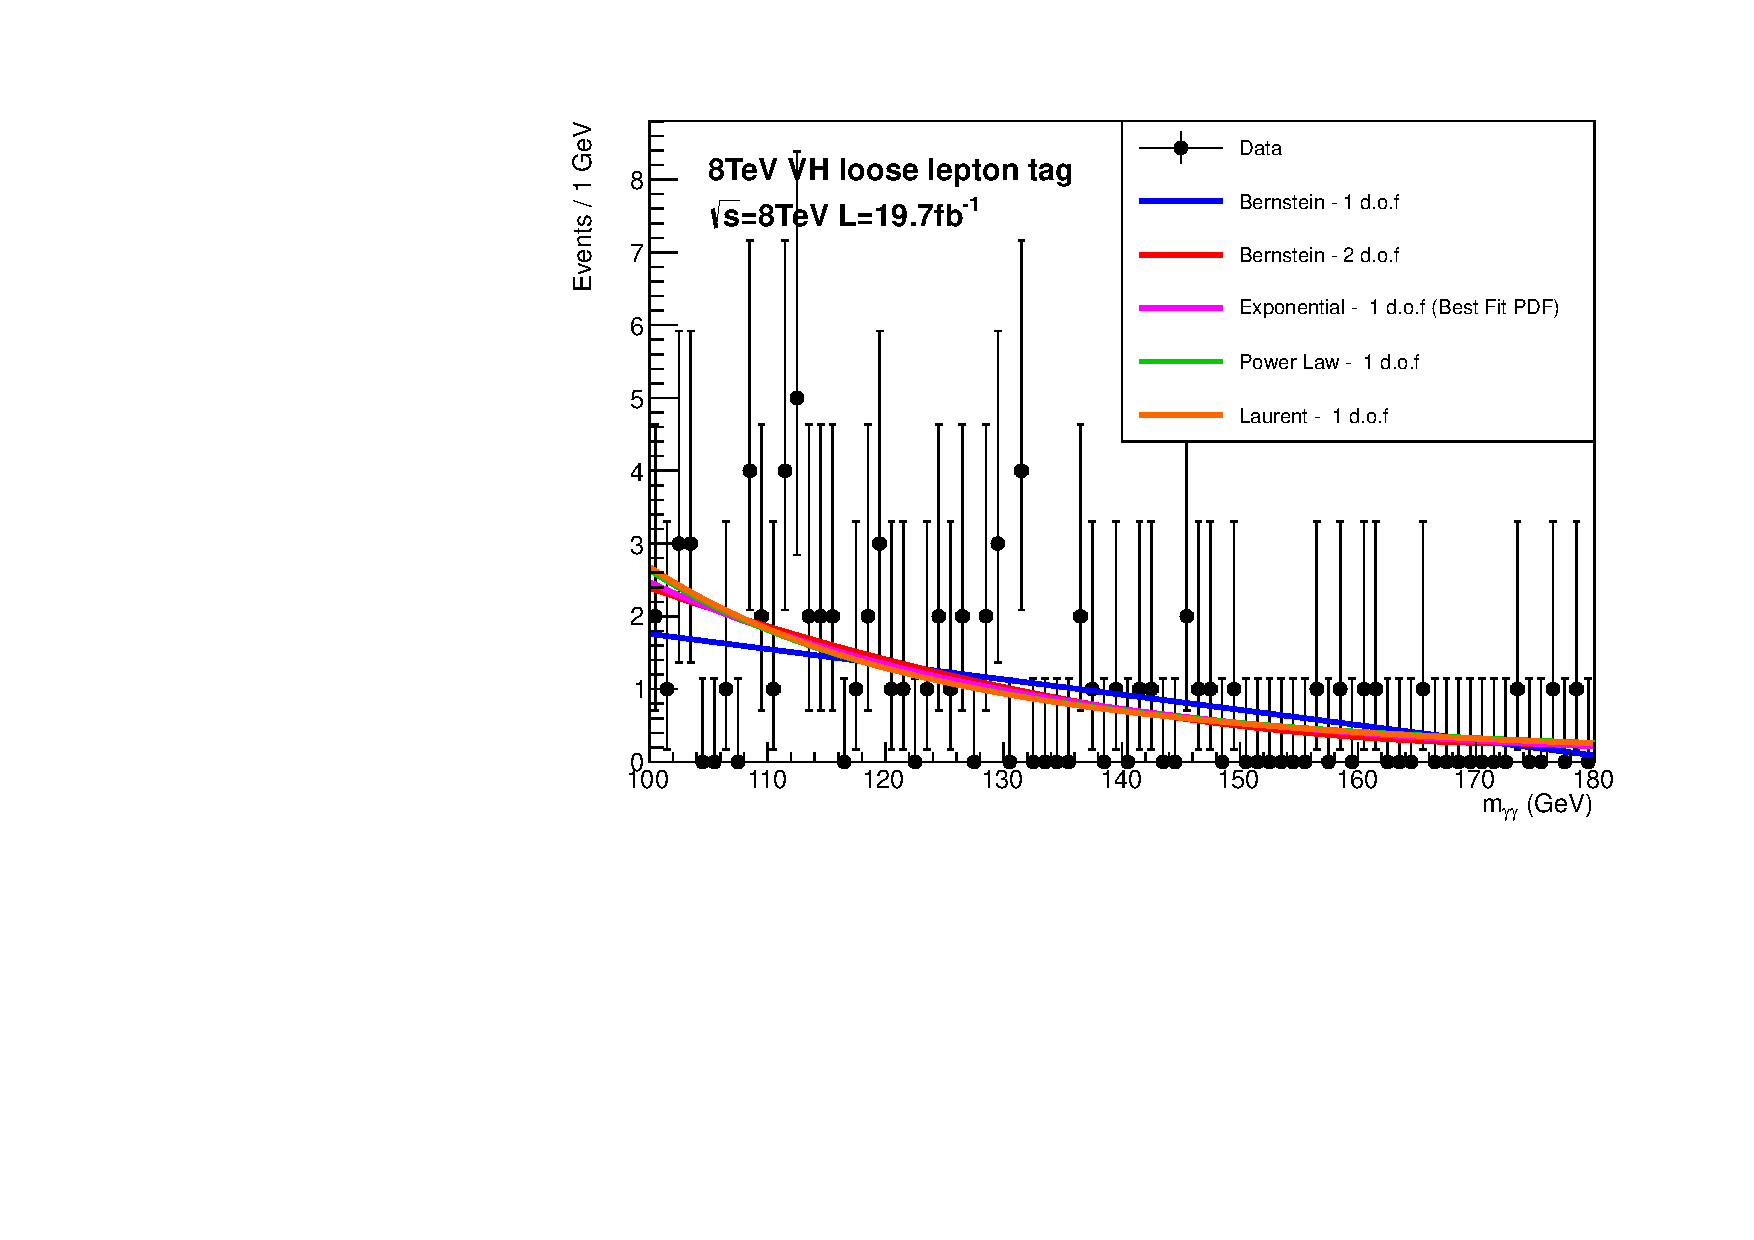
\includegraphics[width=0.49\textwidth]{analysis/plots/multipdf_plots/cat9_8TeV.pdf}\\
  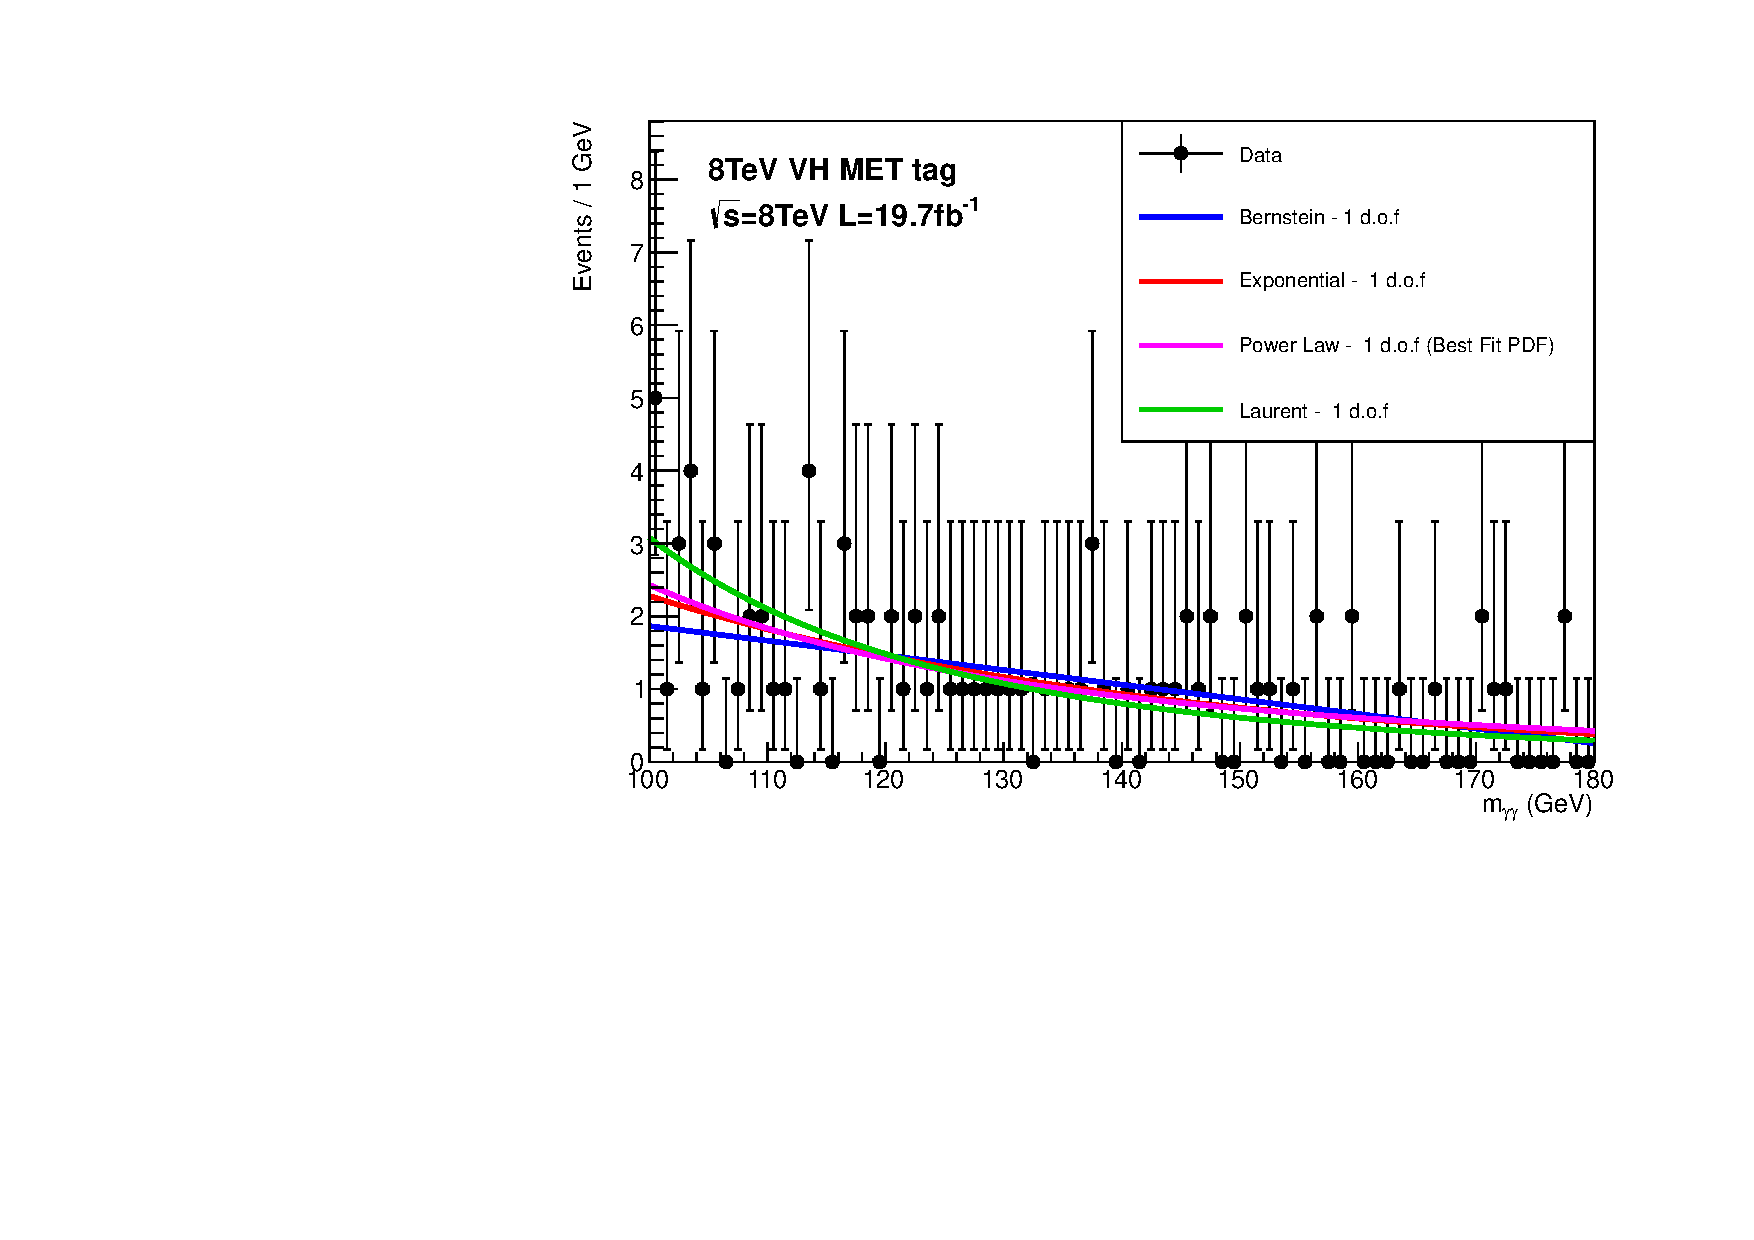
\includegraphics[width=0.49\textwidth]{analysis/plots/multipdf_plots/cat10_8TeV.pdf}
  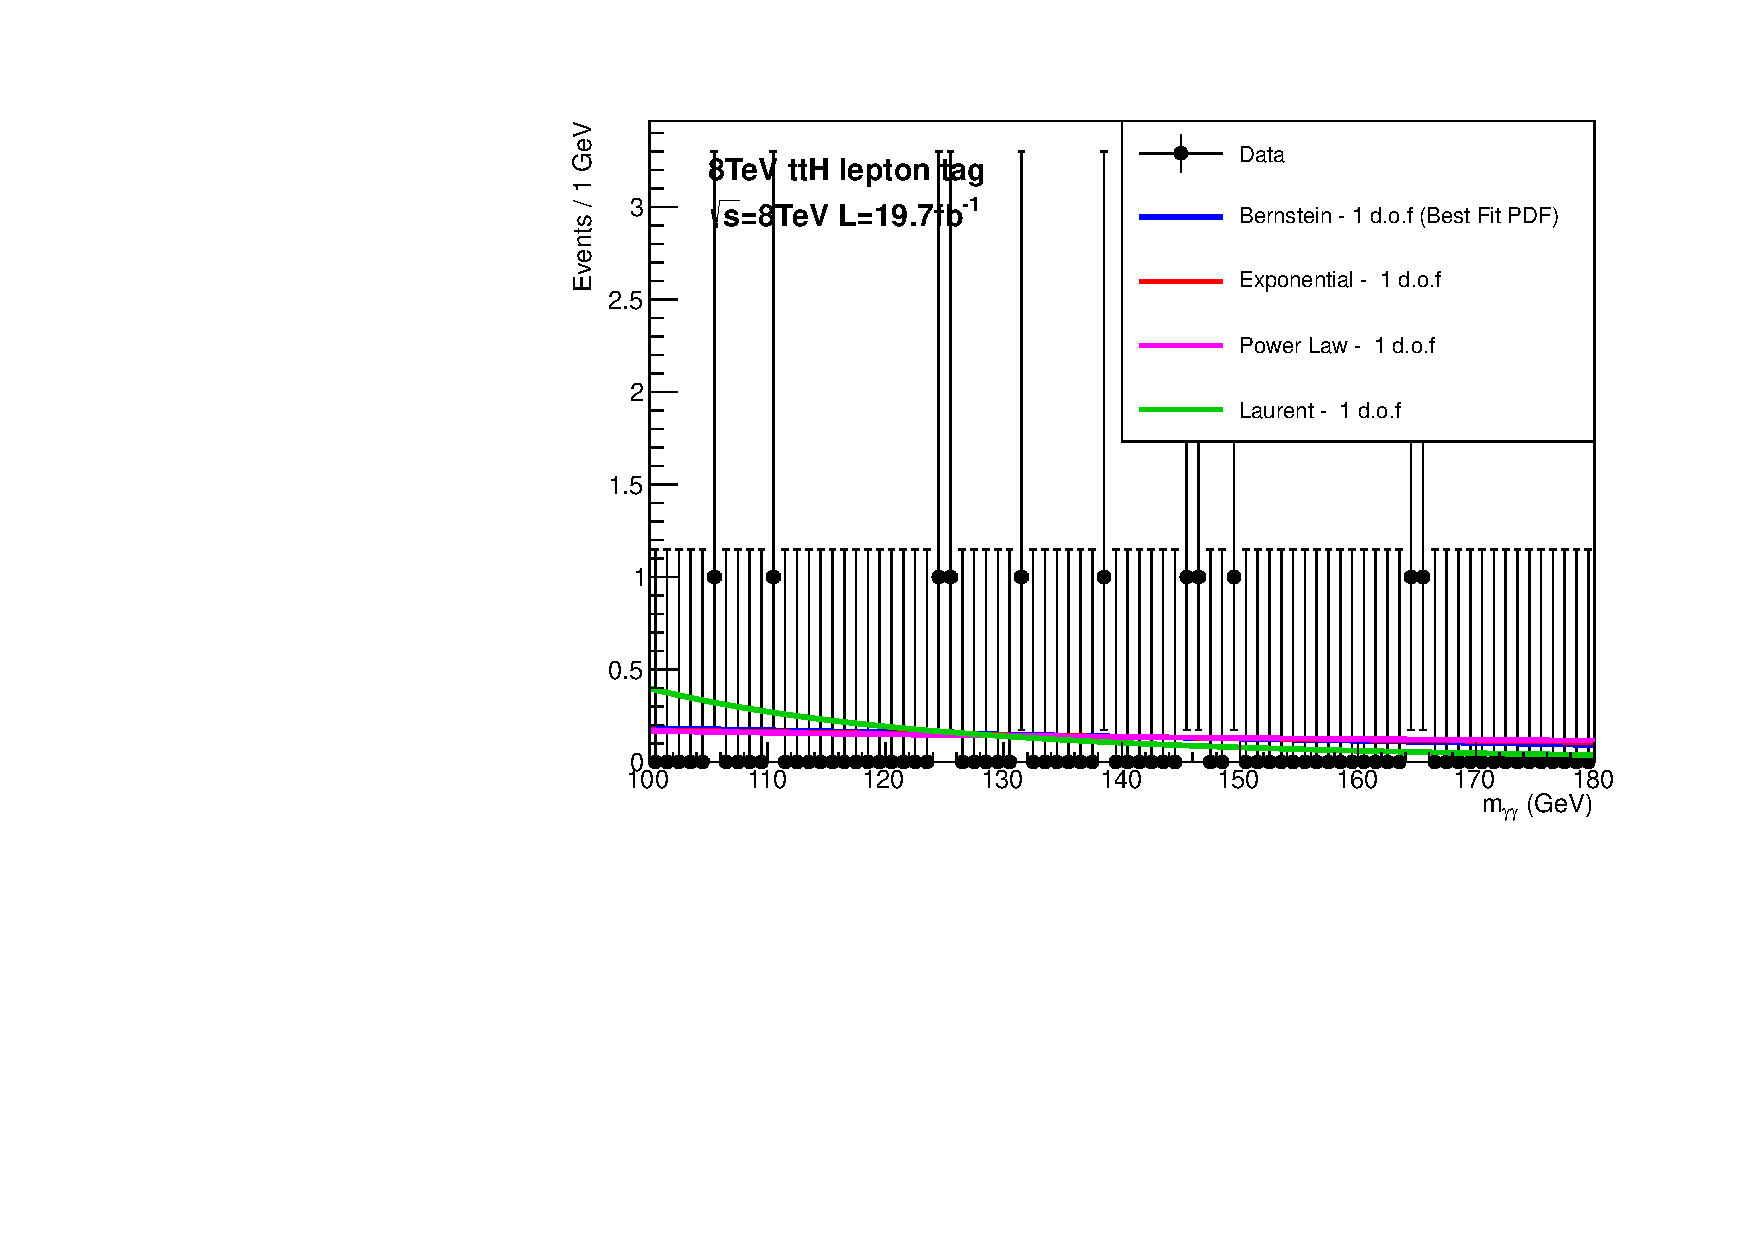
\includegraphics[width=0.49\textwidth]{analysis/plots/multipdf_plots/cat11_8TeV.pdf}\\
  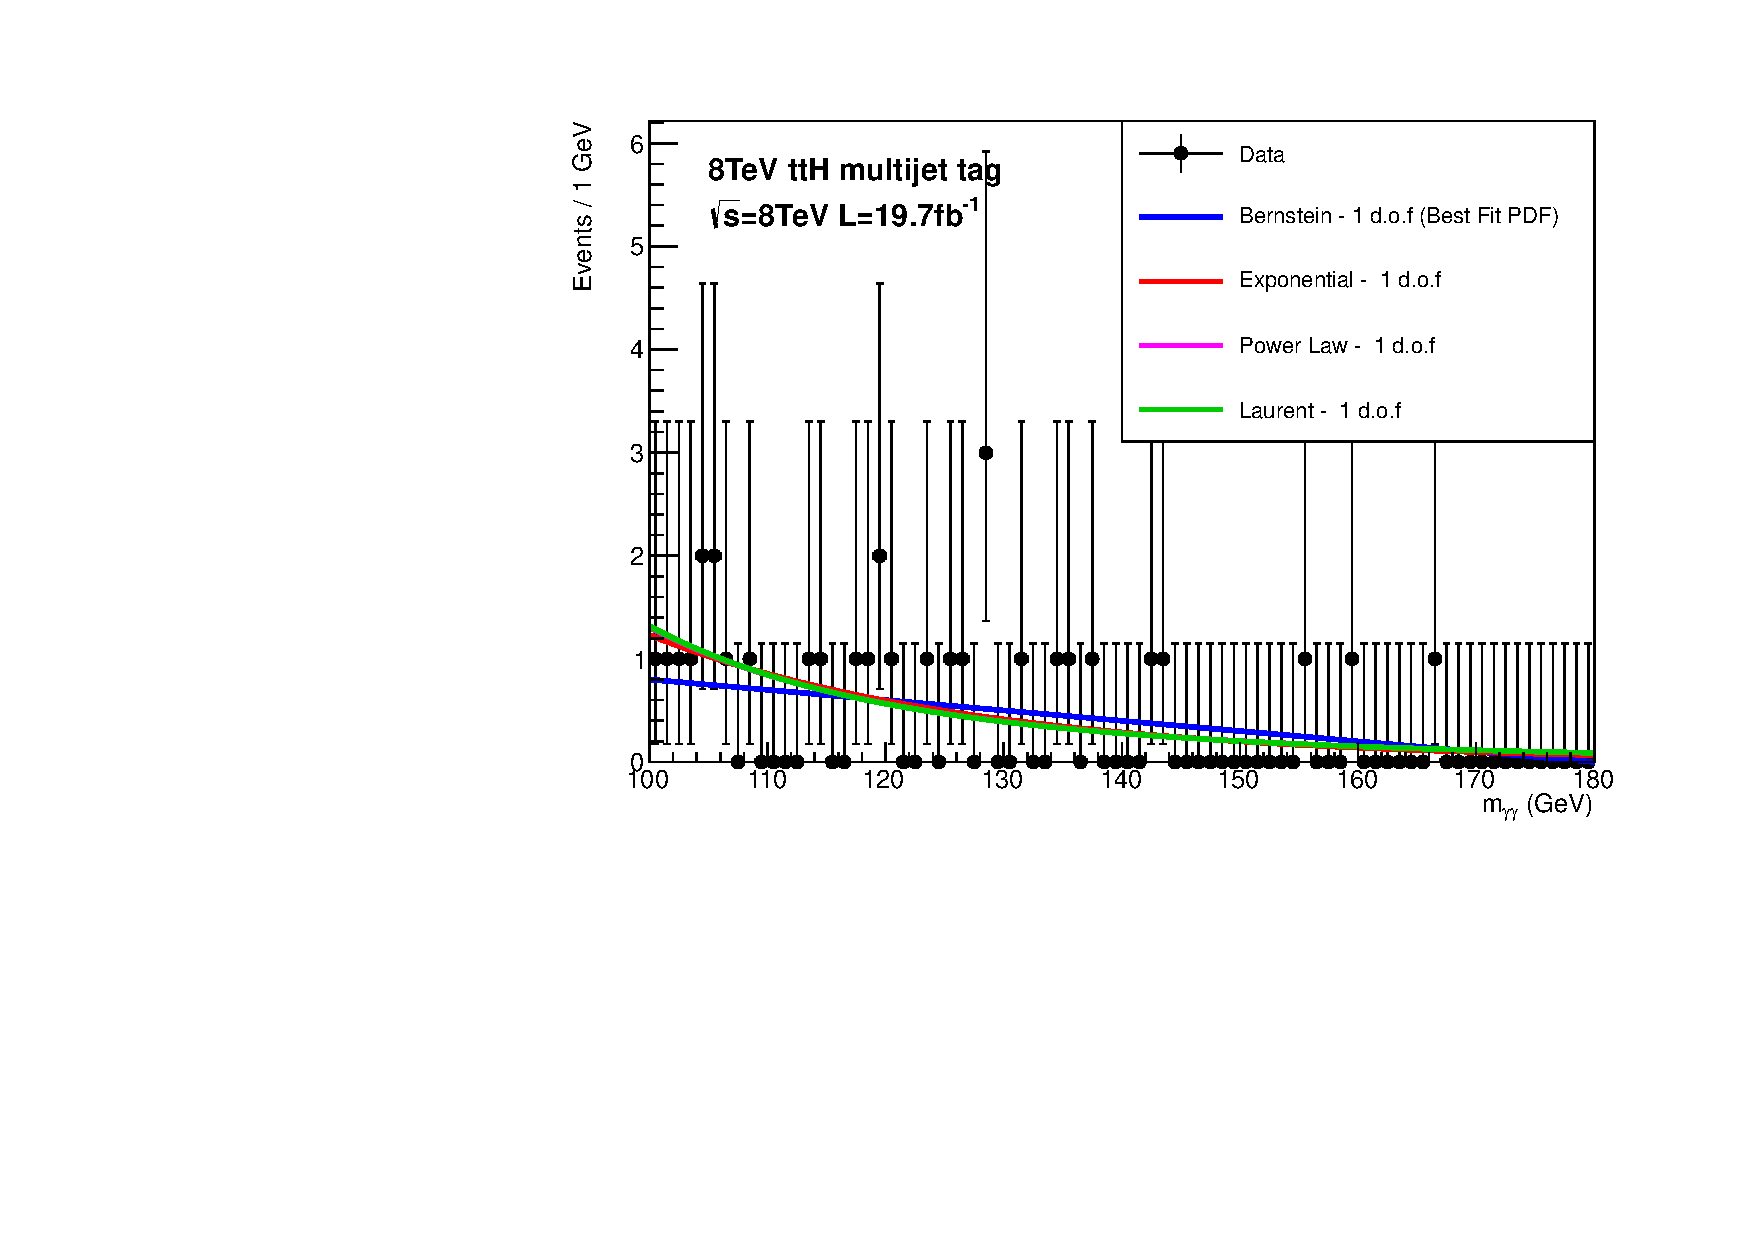
\includegraphics[width=0.49\textwidth]{analysis/plots/multipdf_plots/cat12_8TeV.pdf}
  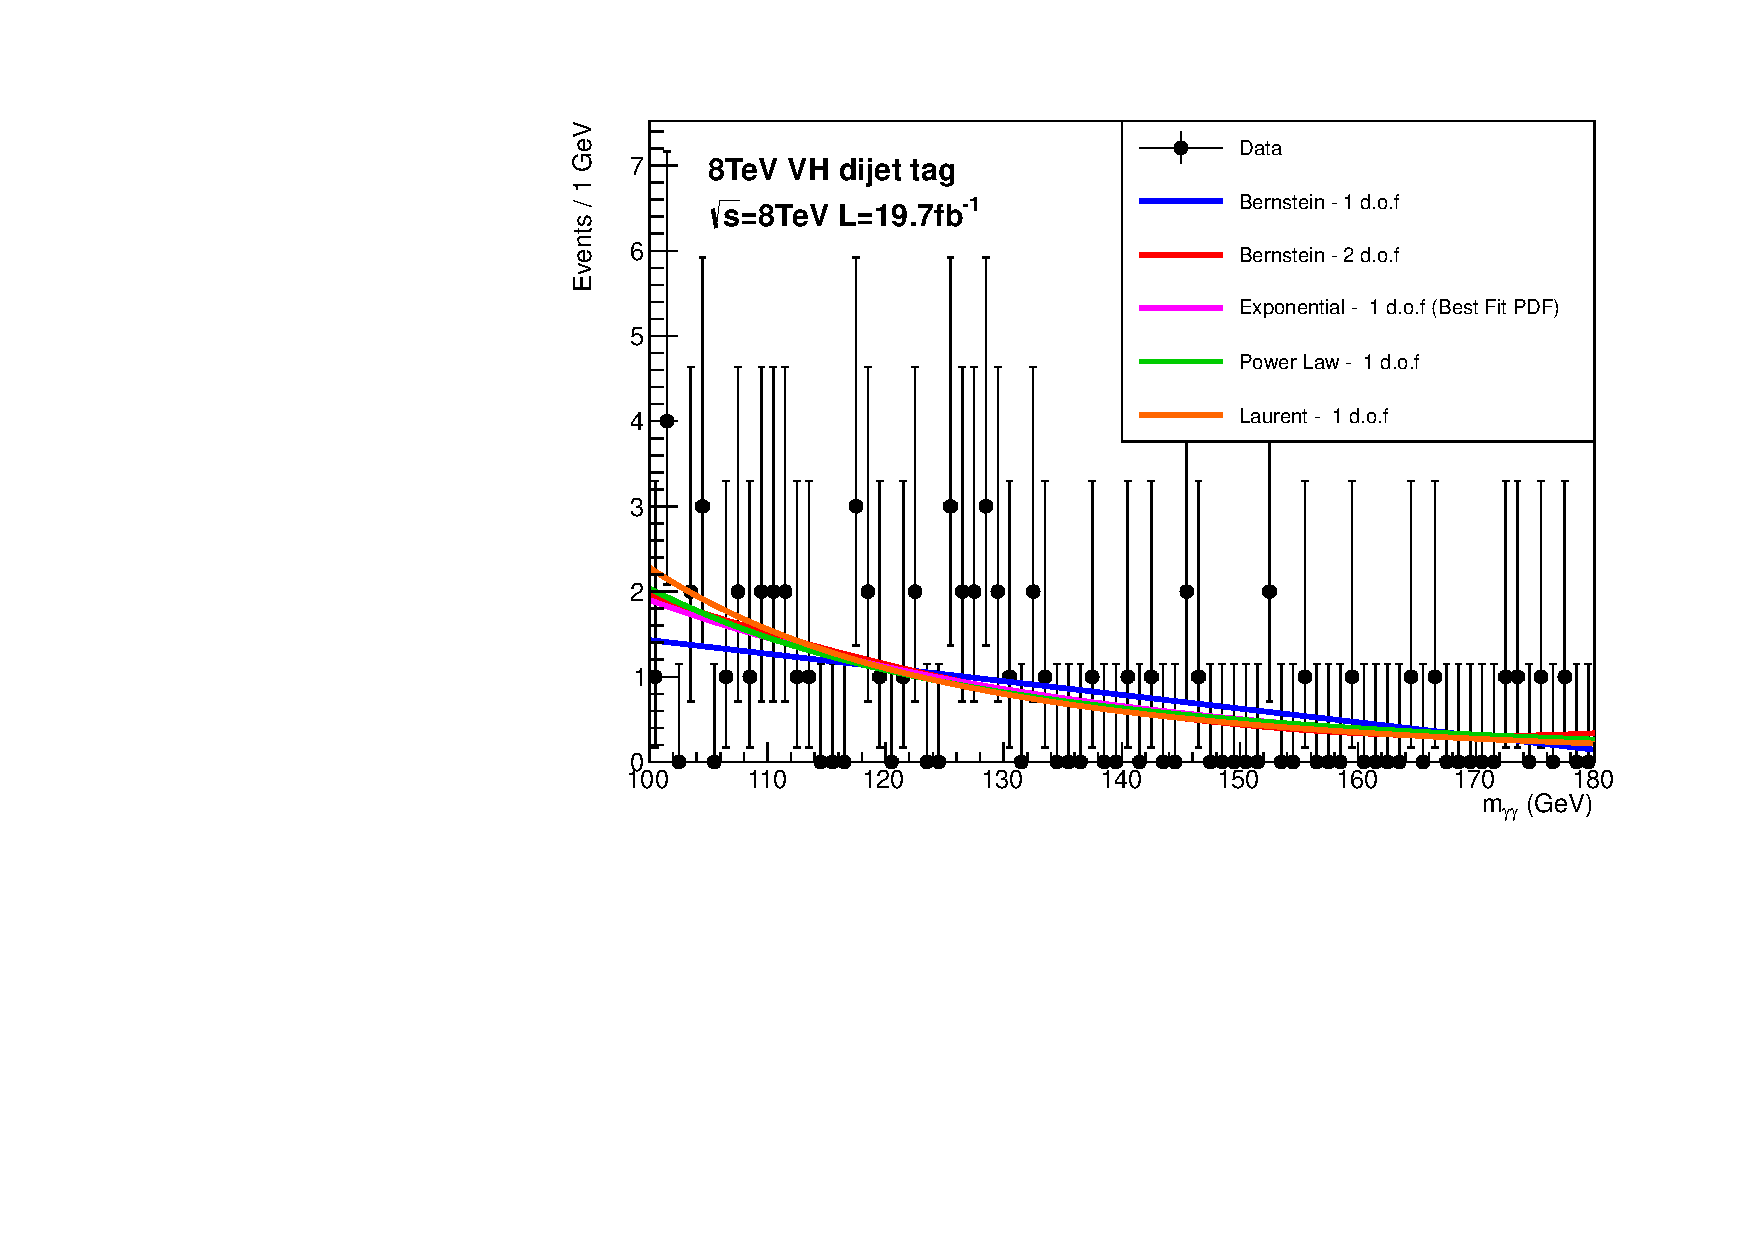
\includegraphics[width=0.49\textwidth]{analysis/plots/multipdf_plots/cat13_8TeV.pdf}
  \caption{The diphoton invariant mass distribution and the background function choices profiled using the envelope method for the \VH and \ttH tag categories in the 8~\TeV dataset.}
  \label{fig:multipdf4}
\end{figure}

